%-----------------------------------------------------------------------------%
% Este es el trabajo de tesis de Itzel Isunza Manrique (itzimah@gmail.com).   %
% Está basada en una plantilla por Sean Anderson (github.com/roguephysicist). %
%-----------------------------------------------------------------------------%

\documentclass[letterpaper,11pt,openany,oneside]{book}

\usepackage{xmpincl}% For including licensing XMP metadata
\usepackage{amsmath}% AMS Math
\usepackage{amssymb}% AMS Symbol
\usepackage{parskip}% No indent, line skipping paragraph breaks
\usepackage{float}% For better control of figure placement and additional floats
\usepackage{caption}

\usepackage{fancyhdr}% Fancy headers and footers.
\pagestyle{empty}% Empty for \frontmatter

\usepackage{graphicx}% You know it, baby!
\graphicspath{{.}{content/images/}}

\usepackage{color}% For link colors
\definecolor{linkcol}{rgb}{0,0,0.4} 
\definecolor{citecol}{rgb}{0.5,0,0}
\definecolor{emerald}{rgb}{0,0.5,0.5}

\usepackage[bookmarksdepth=2,colorlinks=true,linkcolor=linkcol,citecolor=citecol,filecolor=magenta,urlcolor=linkcol,breaklinks=true]{hyperref}
\urlstyle{same}% For all links within the document and URLs

\usepackage{minitoc}% Mini table of contents for each chapter
\setcounter{minitocdepth}{2}

\usepackage[nottoc,notlof,notlot]{tocbibind}% Fine tuning table of contents
\setcounter{tocdepth}{2}% Number of levels shown in TOC
\setcounter{secnumdepth}{3}% Levels of section numbering
\addtocontents{toc}{\protect\thispagestyle{empty}}% Ensures no page
\addtocontents{lof}{\protect\thispagestyle{empty}}% numbers on toc,
\addtocontents{lot}{\protect\thispagestyle{empty}}% lof, or lot

%------------------------------ Definitions --------------------------------%
% Centered page environment for frontmatter.
% Credit to Matthieu Herrb (matthieu@laas.fr)
\newenvironment{vcenterpage}
{\newpage\vspace*{\fill}\thispagestyle{empty}\renewcommand{\headrulewidth}{0pt}}
{\vspace*{\fill}}

% Changes line spacing to be slightly easier to read
%\renewcommand{\baselinestretch}{1.05}

% Modifies book class defaults for better looking
% chapter pages with small caps titles
\makeatletter
\def\@makechapterhead#1{%
  \vspace*{1\p@}%
  {\parindent \z@ \raggedright \normalfont
    \ifnum \c@secnumdepth >\m@ne
      \if@mainmatter
        \LARGE\sc \@chapapp\space \thechapter
        \par\nobreak
        \vskip 10\p@
      \fi
    \fi
    \interlinepenalty\@M
    \Huge \sc #1\par\nobreak
    \vskip 25\p@
  }}
\def\@makeschapterhead#1{%
  \vspace*{1\p@}%
  {\parindent \z@ \raggedright
    \normalfont
    \interlinepenalty\@M
    \Huge \sc  #1\par\nobreak
    \vskip 30\p@
  }}
\makeatother
% Packages and new defintions
\hypersetup{% PDF display options
    pdftitle={Emision de luz en sistemas organicos nanoestructurados y funcionalizados},
    pdfauthor={Itzel Isunza Manrique},
    pdfsubject={Trabajo de tesis de Itzel Isunza Manrique.},
    pdfkeywords={nanoparticulas} {nolineal} {optica} {organico} {tesis} {licenciatura}}
  
\usepackage[lmargin=1.8in,rmargin=1.4in]{geometry}    
\usepackage[T1]{fontenc}% T1 font encoding for special characters.
\usepackage{lmodern}% Better Latin Modern font.
\usepackage[latin1]{inputenc}
\usepackage{layout}
\usepackage{subcaption}
\usepackage[spanish,activeacute,es-nosectiondot]{babel}
\decimalpoint

\addto\captionsspanish{\renewcommand{\tablename}{Tabla}}

%\usepackage{draftwatermark}% Add watermark to background
%\SetWatermarkText{DRAFT}
%\SetWatermarkScale{2}
%\SetWatermarkLightness{0.87}
%\SetWatermarkFontSize{2cm}

%\usepackage{showkeys}% Shows all \label values for quick troubleshooting
%\includeonly{}% Select individual chapters for quicker drafts

%\addtolength{\voffset}{-0.96cm} 
%\addtolength{\hoffset}{0.9cm}

\begin{document}
\mtcselectlanguage{spanish2}
\dominitoc

%\renewcommand{\contentsname}{Contenido}
%\layout %% para tener los valores del margen y por si los quieres cambiar, esto por si no te dejan imprimir la tesis en las dos paginas de una hoja

\frontmatter
%\addtolength{\hoffset}{-0.5cm}
\begin{titlepage}
\begin{center}
  %\newcommand{\Ptitle}{Emisi\'on de luz en sistemas org\'anicos nanoestructurados y funcionalizados}

   
  
   
  %\rightline{
\includegraphics[scale=.95]{frontmatter/escudoUGTO.png}}   \leftline{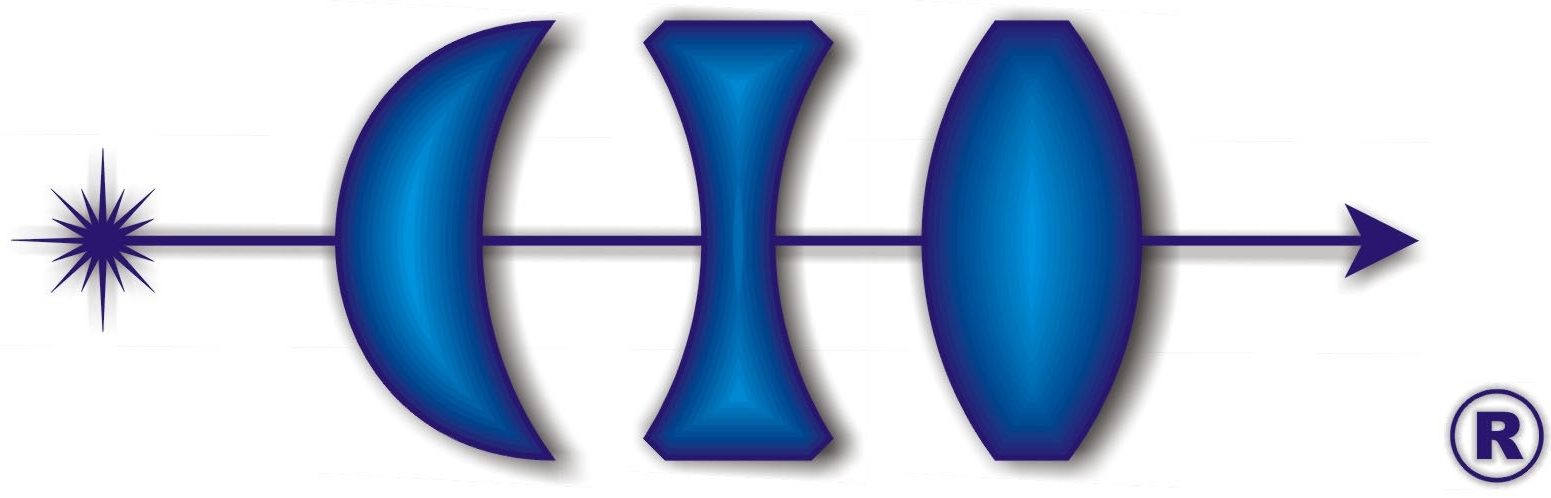
\includegraphics[scale=.41]{frontmatter/logo.png}} }
   
   {
  % \vspace{1.4cm}

{\large Centro de Investigaciones en \'Optica, A. C. }\\   
    \vspace{.6cm}
    
    \large Universidad de Guanajuato\\
   %     \vspace{.4cm}
%\large Divisi�n de Ciencias e Ingenier�as
        \vspace{.8cm}


 \begin{figure}%[!htb]
\minipage{0.37\textwidth}
 \rightline{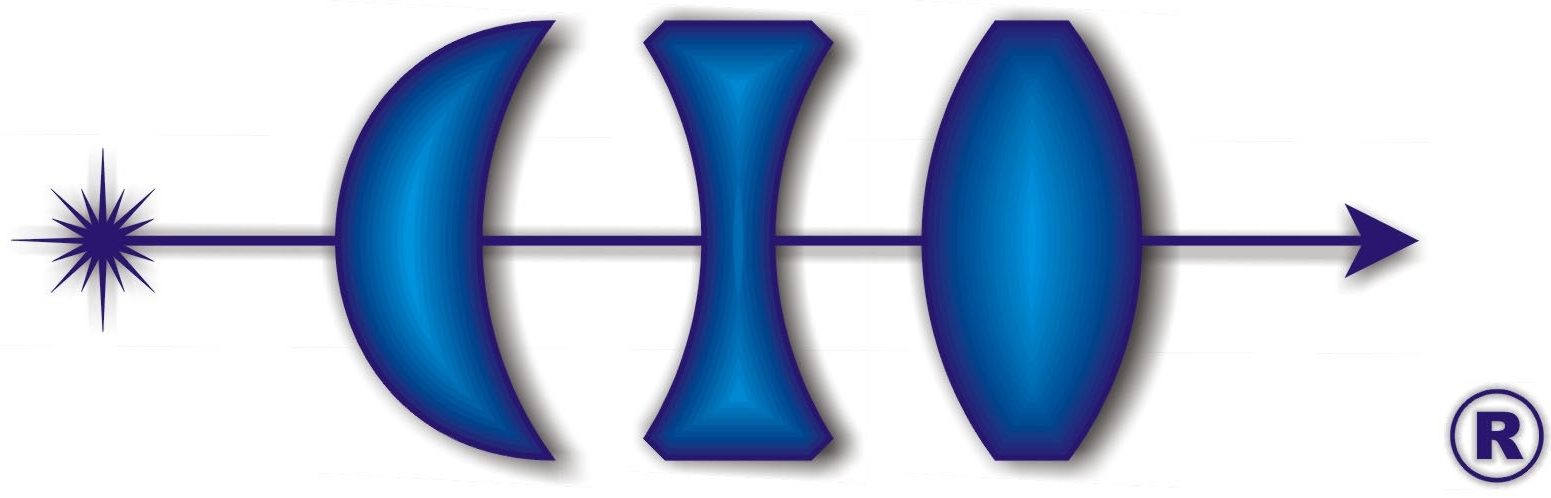
\includegraphics[scale=.38]{frontmatter/logo.png}}
\endminipage\hfill
\minipage{0.16\textwidth}
  \leftline{
\includegraphics[scale=.83]{frontmatter/escudoUGTO.png}}
\endminipage
\end{figure}



    \vspace{0.6cm}


{\LARGE  Emisi\'on de luz en  \vspace{0.2cm}sistemas org\'anicos nanoestructurados  \vspace{0.2cm}y funcionalizados\\
\vspace{0.6cm}


{\large{por}}
\vspace{0.3cm}

{\LARGE {Itzel Isunza Manrique}}
%\vspace{0.3cm}
}

\vspace{0.8cm}

    {\large Tesis para obtener el t\'itulo de Licenciada en F\'isica\\}

    



\vspace{0.9cm}

{\large Asesor:}
\vspace{0.4cm}
{\large\\Dr. Gabriel Ramos Ortiz\\}
\vspace{0.6cm}
{\large Co- Asesor:}
\vspace{0.4cm}
{\large\\Dr. Teodoro C�rdova Fraga}


\vfill
\vspace{0.6cm}
\large{Julio 2014}
}
\end{center}
\end{titlepage}

 %esta es del cio ug
%\addtolength{\hoffset}{-1.6cm}
\begin{vcenterpage}
{\LARGE{\sc Resumen}}
%\chapter*{Resumen}

\noindent\rule[2pt]{\textwidth}{0.5pt}
En este trabajo se presenta un estudio de las propiedades \'opticas m\'as relevantes de nuevos sistemas moleculares org\'anicos para el desarrollo de marcadores biocompatibles en microscop\'ia de fluorescencia.

Se realiz\'o una comparaci\'on entre la actividad \'optica de estos materiales en soluci\'on y en suspensiones acuosas de nanopart\'iculas, fabricadas mediante el m\'etodo de reprecipitaci\'on. Para ello se obtuvieron espectros de absorci\'on en el rango UV-visible y espectros de emisi\'on lineal utilizando una fuente de excitaci\'on de 370 nm. Se determinaron adem\'as los valores de eficiencia cu\'antica de fluorescencia utilizando una esfera integradora. 

Adicionalmente se obtuvieron los valores de secci\'on transversal de absorci\'on de dos fotones en el rango de inter\'es biom\'edico (740- 840$nm$ y 650- 760$nm$) mediante la t\'ecnica de emisi\'on inducida por absorci\'on de dos fotones, TPEF por sus siglas en ingles. En el rango de 740 a 840 $nm$ se utiliz\'o un l\'aser de Ti: Za con pulsos de 100 $fs$ y frecuencia de repetici\'on de 80 $MHz$; para longitudes de onda de 650 a 760 nm se utiliz\'o un amplificador ultrarr\'apido con emisi\'on de pulsos de 50 $fs$ y frecuencia de 1 $kHz$.
	
Por otra parte, se realizaron estudios para desarrollar y optimizar una transferencia de energ�a de resonancia F�rster en suspensiones acuosas de nanopart�culas, realizando posteriormente una caracterizaci�n �ptica.  	
	
Se desarroll\'o una metodolog\'ia para la fabricaci\'on de nanopart\'iculas org\'anicas funcionalizadas con dos tipos de Polietilenglicol (PEG) y se estudiaron efectos en las propiedades \'opticas. Las nanopart\'iculas funcionalizadas que presentaron propiedades fluorescentes y que resultaron de mayor inter\'es se sometieron a un estudio de fotoestabilidad para finalmente ser internalizadas en c\'elulas epiteliales L929 y obtener im\'agenes (micro- im\'agenes) con un microscopio de epifluorescencia.


\noindent\rule[2pt]{\textwidth}{0.5pt}
\end{vcenterpage}

%\begin{vcenterpage}
{\LARGE{\sc Dedication}}

\noindent\rule[2pt]{\textwidth}{0.5pt}

Lorem ipsum dolor sit amet, consectetur adipiscing elit. Sed libero elit, sollicitudin dignissim accumsan aliquam, eleifend et massa. 

\noindent\rule[2pt]{\textwidth}{0.5pt}
\end{vcenterpage}

\begin{vcenterpage}
\newpage
{\LARGE{\sc Agradecimientos}}

\noindent\rule[2pt]{\textwidth}{0.5pt}
\small{	
Agradezco al Centro de Investigaciones en \'Optica por brindarme la oportunidad de desarrollar este trabajo. En particular, agradezco al Grupo de Propiedades \'Opticas de la Materia (GPOM) y a sus integrantes por el apoyo y retroalimentaci\'on.  

Tambi\'en agradezco a las personas que proporcionaron los materiales de estudio que aqu� se presentan: a la M.C. Mariana Flores y al Dr. Alejandro Alvarez de la Universidad Aut\'onoma del Estado de Hidalgo, al Dr. Ullrich Scherf de Bergische Universit\"at Wuppertal, a la Dra. Rosa Santill\'an y Dr. Arturo Jim\'enez del Cinvestav- IPN; en especial agradezco a Arturo por su ayuda y apoyo constante. 

Agradezco a la Dra. Myrna Sabanero y a sus estudiantes del Laboratorio de Biolog\'ia Celular y Molecular de las Interacciones de la UG por el apoyo para llevar a cabo la internalizaci\'on de nanopart\'iculas en las c\'elulas. Agradezco su paciencia y sobre todo sus ense�anzas. 

A Leonardo P�rez por su amistad y en particular por el apoyo para la adquisici\'on de im�genes con el microscopio de epifluorescencia del CIO.

Tambi\'en agradezco al Ing. f\'isico Manuel De Anda por su ayuda y capacitaci�n brindada para trabajar con el amplificador ultrarr�pido y otros equipos, agradezco la paciencia mostrada y amistad. 

Agradezco a mis compa�eros y amigos por la ayuda brindada durante todo este tiempo, en especial a \'Alvaro Romero, Enrique Alba, Daniel L�pez, Jonathan P�rez, Mart�n Olmos, Misael Barba, Ari�n Roa y Luis Lozano. Tambi�n agradezco a Sean Anderson por su amistad y por el invaluable apoyo mostrado durante la elaboraci�n de este trabajo.

A mi tutor Teodoro Cordova por la disposici�n tan entusiasta que siempre tuvo por ayudarme y el inter�s mostrado durante mi formaci�n acad�mica.

Agradezco de una manera muy especial, a Laura Aparicio por sus ense�anzas dentro del laboratorio y fuera de el, por su paciencia y disposici�n que siempre tuvo para ayudarme en todo momento.

Mis m�s grandes agradecimientos son para mi asesor de tesis Gabriel Ramos, por haberme otorgado esta gran oportunidad de aprender, por el invaluable apoyo y atenci�n que siempre me mostr�, por sus correcciones y sobre todo sus ense�anzas.

Finalmente agradezco a mi familia, por ser un soporte incondicional en mi vida, en especial agradezco a mi madre y a mi abuela por todo su apoyo y comprensi\'on durante todos estos a�os.
}

\noindent\rule[2pt]{\textwidth}{0.5pt}
\newpage
\end{vcenterpage}
 % AGRADECIMIENTOS!!!!!!!!!

\tableofcontents
\listoffigures
%\listoftables

\mainmatter
% Fancy header style options for each page
\pagestyle{fancy}% Sets fancy header and footer
\fancyhead{}% Resets headers
\fancyfoot{}% and footers

\fancyhead[LE,RO]{\thepage}% Page number left on even and right on odd pages
\fancyhead[RE]{\itshape\nouppercase{\leftmark}}% Chapter right on even pages
\fancyhead[LO]{\itshape\nouppercase{\rightmark}}% Section left on odd pages
\renewcommand{\headrulewidth}{0.5pt}

\fancypagestyle{plain}{
  \fancyhead{}
  \fancyfoot{}
  \renewcommand{\headrulewidth}{0pt}
}

% No headers on empty pages before new chapter
\makeatletter
\def\cleardoublepage{\clearpage\if@twoside \ifodd\c@page\else
    \hbox{}
    \thispagestyle{plain}
    \newpage
    \if@twocolumn\hbox{}\newpage\fi\fi\fi}
\makeatother \clearpage{\pagestyle{plain}\cleardoublepage}

\chapter{Introducci\'on}\label{chap_intro}
\minitoc

\section{Biofot\'onica y nuevos m\'etodos de adquisici\'on de im\'agenes}

Uno de los avances cient\'ificos m\'as importantes del siglo \textrm{XXI} es la biofot\'onica, estudio multidisciplinario que integra cuatro tecnolog\'ias: l\'aseres, fot\'onica, nanotecnolog\'ia y biotecnolog\'ia. 

La biofot\'onica fusiona ciencias biom\'edicas con la fot\'onica y estudia interacciones entre la luz y sistemas biol\'ogicos. Cuando esta definici\'on se toma en el sentido en el que la fot\'onica se aplica en ciencias biom\'edicas, la biofot\'onica busca resolver problemas de salud en \'areas de oncolog\'ia, dermatolog\'ia, oftalmolog\'ia, cirug\'ia y cardiolog\'ia; presentando nuevas modalidades de terapias basadas en luz guiada y activadas por luz, y alternativas para la detecci\'on temprana de enfermedades.

En la figura \ref{cuadro_intro} se muestra un panorama general de las aplicaciones en biofot\'onica para el cuidado de la salud. Se han desarrollado tratamientos que simplifican la entrega de medicamentos en sitios de inter\'es y terapias capaces de destruir c\'elulas cancer\'igenas, as\'i como el desarrollo de diagn\'osticos confiables basados en diversas t\'ecnicas y dispositivos que realizan un estudio estructural de c\'elulas y tejidos.

Un \'area fundamental de la biofot\'onica est\'a enfocada en la adquisici\'on de im\'agenes $in$ $vivo$ e $in$ $vitro$ de espec\'imenes o muestras biol\'ogicas utilizando m\'etodos \'opticos. Las t\'ecnicas que se encargan de monitorear propiedades \'opticas para formar una imagen, se basan principalmente en el an\'alisis de fluorescencia, transmisi\'on y reflexi\'on de la luz, como la tomograf\'ia de coherencia \'optica, espectroscop\'ia y microscop\'ia. 

\begin{figure}[h]
\centering
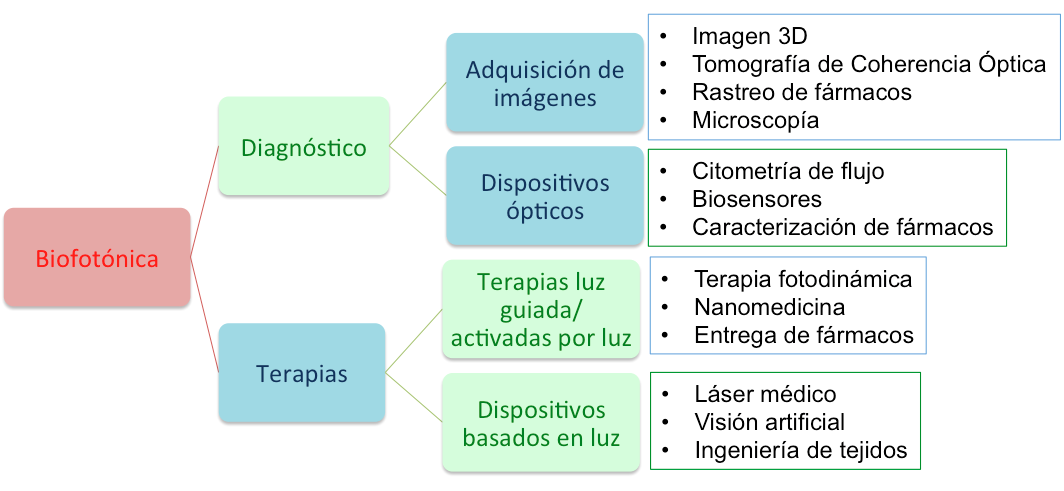
\includegraphics[width=1\textwidth]{c1_Introduction/intro}
\caption{Alcance multidisciplinario de la Biofot\'onica en el cuidado de la salud \label{cuadro_intro}}
\end{figure}

%Por ejemplo, en la terapia fotodin\'amica se utiliza un agente qu\'imico o fotosensibilizador que al ser activado por luz destruye c\'elulas cancer\'igenas; en relaci\'on a tratamientos m\'edicos, se han desarrollado portadores de f\'armacos, que con ayuda de la nanotecnolog\'ia simplifican la entrega de medicamentos en ciertos sitios de inter\'es. Y enfocadas en el diagn\'ostico, hay t\'ecnicas en las que se utilizan marcadores fluorescentes como citometr\'ia de flujo, espectroscop\'ia de fluorescencia y dispositivos como biosensores \'opticos que pueden realizar desde un estudio estructural de c\'elulas y tejidos hasta una detecci\'on temprana de c\'ancer.

En la actualidad la microscop\'ia ha sido ampliamente utilizada debido a las im\'agenes de mayor resoluci\'on y contraste que se pueden adquirir en comparaci\'on con otras t\'ecnicas convencionales. La microscop\'ia combina e implementa t\'ecnicas como la microscop\'ia confocal, microscop\'ia de barrido y microscop\'ia de fluorescencia; adem\'as se han desarrollado microscopios basados en procesos de \'optica no lineal como la microscop\'ia de segundo o tercer arm\'onico y multifot\'on.

El desarrollo de nuevos materiales biocompatibles ha contribuido con el avance de algunas aplicaciones en biofot\'onica. Ha impulsado tratamientos, terapias y m\'etodos de diagn\'ostico, con el uso de fotosensibilizadores, portadores de f\'armacos y agentes qu\'imicos. Particularmente ha sido fundamental en t\'ecnicas de microscopia que involucran el an\'alisis de fluorescencia por el uso de compuestos qu\'imicos ex\'ogenos como marcadores en especies biol\'ogicas.

%Entre los cuales se pueden citar colorantes comerciales, nanopart\'iculas inorg\'anicas, puntos cu\'anticos y recientemente, nanoparticulas org\'anicas utilizando nuevos pol\'imeros conjugados y mol\'eculas de tama\~{n}os variables con propiedades de inter\'es.

%La carcterizaci\'on \'optica de los nuevos materiales se seleccionan cuales de ellos pueden utilizarse para solucionar problemas espec�ficos en la adquisicionnn de la imagen e s

%Se han utilizado como marcadores biocompatibles 
%no me importa esto%%%%%%%%%%%%%%\textcolor{emerald}{\sffamily This manual was made using the template that you just downloaded. All the source files are included so you can recompile, modify, and deconstruct any part of it. Text that is this color and style indicates that I am talking about this document you are reading. I believe in learning by doing \cite{oetiker2011not} so I suggest you follow along and review the source code while reading.}

\section{Antecedentes: Marcadores en microscop\'ia de fluorescencia}

Durante el siglo XVII  se llev\'o a cabo la primera observaci\'on de c\'elulas con un microscopio \'optico, desde entonces el desarrollo de nuevas t\'ecnicas y dispositivos para la obtenci\'on de im\'agenes con mayor resoluci\'on no se hizo esperar. En 1911 el f\'isico Oskar Heimst\"adt (tras el desarrollo del primer microscopio UV por August K\"ohler) construy\'o el primer microscopio de fluorescencia con el cual se visualiz\'o una bacteria \cite{revistanature}. A pesar de ello, este microscopio ten\'{\i}a una fuerte limitante: la obtenci\'on de im\'agenes depend\'{\i}a de la autofluorescencia o fluorescencia end\'ogena de los objetos.

Para ampliar los alcances de este microscopio, el austriaco Max Haitinger desarroll\'o una t\'ecnica de fluorescencia secundaria o ex\'ogena la cual implicaba el uso de qu\'{\i}micos que induc\'{\i}an fluorescencia en las muestras. En 1934 Haitinger acu\~{n}\'o el t\'ermino \emph{fluorocromo}  para referirse a estos colorantes fluorescentes \cite{libro}, aunque hoy en d\'{\i}a se conocen tambi\'en como fluor\'oforos. 

Sin embargo, el descubrimiento m\'as importante en el campo de microscop\'ia de fluorescencia se llev\'o a cabo en 1941 por Albert Coons: la inmunofluorescencia \cite{libro}. Esta t\'ecnica  permite localizar biomol\'eculas espec\'{\i}ficas en c\'elulas o tejidos, adhiriendo un colorante fluorescente a un anticuerpo (Ver Figura \ref{celfluo}). Coons localiz\'o diversos tipos de prote\'inas en c\'elulas, adhiriendo una sustancia org\'anica hidrosoluble conocida como fluoresce\'ina a un anticuerpo.


\begin{figure}[ht]
\centering
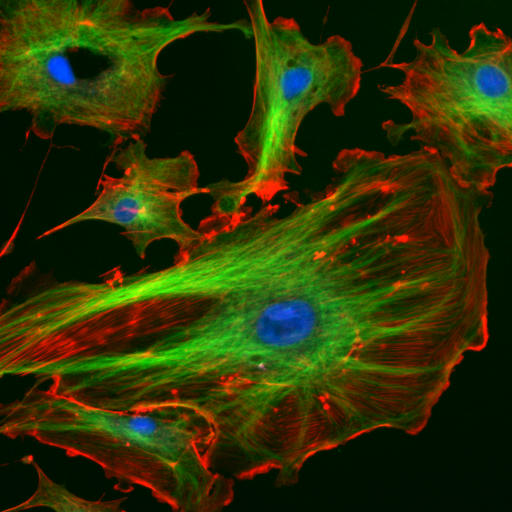
\includegraphics[width=3.2in, height=2.5in]{c1_Introduction/FluorescentCells}
\caption{\small{C\'elulas endoteliales bajo microscopio de fluorescencia. En azul, el n\'ucleo te\~{n}ido con el colorante DAPI, en verde y rojo, los microt\'ubulos y filamentos de actina te\~{n}idos por la adhesi\'on de los colorantes FITC y TRITC en anticuerpos.} \emph{\scriptsize{Imagen obtenida de http://rsb.info.nih.gov/ij/images/, sin datos de autor.}}}\label{celfluo}
\end{figure}

Aunque algunas mol\'eculas org\'anicas como la flavina, lipofuscina, prote\'inas y coenzimas, presentan autofluorescencia y pueden ser \'utiles para monitorear procesos celulares; la microscop\'ia de fluorescencia se basa en visualizar, rastrear y/o monitorear la ubicaci\'on o patr\'on de fluorescencia en c\'elulas y tejidos que han sido marcados con fluor\'oforos ex\'ogenos \cite{procons}. 
%En estos casos la autoflorescencia es un problema de ruido que se busca resolver con los m\'etodos  anteriores de microscopia. 



La microscop\'ia de fluorescencia se ha desarrollado en las \'ultimas d\'ecadas con la implementaci\'on de diversos componentes \'opticos y marcadores biocompatibles para obtener im\'agenes de especies biol\'ogicas con resoluci\'on de hasta nan\'ometros. Actualmente hay varios m\'etodos ampliamente utilizados que se basan o pueden basarse en la microscop\'ia de fluorescencia, tales como microscop\'ia de reflexi\'on total interna, confocal,invertida y microscop\'ia de barrido l\'aser de uno y dos fotones entre otras \cite{bioph}.

%Hay un creciente inter\'es en desarrollar materiales que puedan ser utilizados como marcadores fluorescentes sin que afecten la estructura \'o el funcionamiento normal de las c\'elulas y que no causen muerte celular en presencia o ausencia de la fuente de excitaci\'on, es decir que sean marcadores $biocompatibles$.   

\section{Diferentes tipos de marcadores fluorescentes  ?`Por qu\'e utilizar nanopart\'iculas org\'anicas?}
%\subsection{A Note On Operating Systems}
 %\textbf{NEVER} 
 
Hay diversos colorantes comerciales que se pueden utilizar como marcadores biocompatibles, sin embargo, estos tienen limitantes como baja eficiencia cu\'antica de fluorescencia, una tendencia a sufrir r\'apidamente una destrucci\'on fotoqu\'imica conocida como fotoblanqueado (photobleaching en ingl\'es) y principalmente una baja absorci\'on no lineal que dificultan la adquisici\'on de im\'agenes \emph{in vivo} e \emph{in vitro}. Esta \'ultima limitante ha sido la principal motivaci\'on de una de las l\'ineas de investigaci\'on del Grupo de Propiedades \'Opticas de la Materia (GPOM) del Centro de Investigaciones en \'Optica (CIO), la cual ha estado encaminada a desarrollar nuevos materiales con absorci\'on no lineal grande.

Uno de los principales objetivos de la nanotecnolog\'ia aplicada en biofot\'onica  es el uso de nanopart\'iculas como marcadores en sistemas vivos. La nanoqu\'imica es una nueva \'area que se encarga del confinamiento de reacciones qu\'imicas a una escala nanom\'etrica (1 a 100$nm$).  La nanoqu\'imica utiliza un amplio rango de metales, semiconductores, s\'ilice y mol\'eculas y pol\'imeros con sistemas $\pi$ conjugados para la fabricaci\'on de nanopart\'iculas; y puede modificar y funcionalizar la superficie de las mismas.

Un ejemplo son los puntos cu\'anticos, nanopart\'iculas hechas de semiconductores inorg\'anicos cuya ventaja principal es la emisi\'on de luz en un amplio rango de longitudes de onda dependiendo de su tama\~{n}o (Fig.\ref{fig1}). Los puntos cu\'anticos presentan una destrucci\'on fotoqu\'imica casi nula, la  fluorescencia presenta un tiempo de vida prolongado y tienen altos valores de eficiencia cu\'antica de fluorescencia. 
%Esta caracter\'istica se debe a los efectos de confinamiento cu\'antico que se cumplen cuando sus dimensiones son menores que el radio de Bohr \cite{bioph}.
\begin{figure}[ht]
\centering
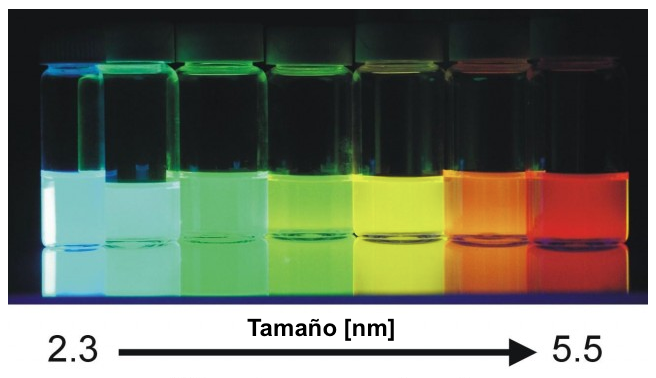
\includegraphics[width=3.2in, height=1.75in]{c1_Introduction/qdots}
\caption{Puntos cu\'anticos. \emph{\scriptsize{Imagen de Benoit Dubertret, 2004}}}\label{fig1}
\end{figure}

A pesar de ser considerados prominentes marcadores para la obtenci\'on de im\'agenes \emph{in vivo} e \emph{in vitro}, las dudas sobre su potencial toxicidad en c\'elulas o \emph{citotoxicidad} a\'un siguen sin resolverse. 

Los puntos cu\'anticos pueden estar limitados por la presencia de metales pesados en su n\'ucleo y bajo ciertas circunstancias pueden ser t\'oxicos para las c\'elulas \cite{artiqdtox}.  Aunque la superficie de estas nanopart\'iculas se puede modificar para aumentar su biocompatibilidad o su eficiencia de emisi\'on, es dif\'icil que el di\'ametro de los puntos cu\'anticos est\'e por debajo del l\'imite de excreci\'on  renal (5.5 nm) y la toxicidad a largo plazo ser\'ia preocupante \cite{articuloQDtoxico}. 
%para adquisici\'on de im\'agenes en sistemas vivos

Otras nanopart\'iculas inorg\'anicas fluorescentes tales como los puntos de carbono, nanopart\'iculas met\'alicas y nanopar\'iculas encapsuladas con s\'ilice, normalmente no son degradables y tienen una potencial toxicidad debido a la acumulaci\'on de estos materiales en el sistema reticuloendotelial \cite{artconcluyente}. 
 
Una alternativa de marcadores fluorescentes que se presenta como soluci\'on a los problemas de citotoxicidad son las nanopart\'iculas basadas en nuevos materiales org\'anicos o con sistemas $\pi$ conjugados: materiales que presentan emisi\'on de luz inducida por agregaci\'on, pol\'imeros conjugados y mol\'eculas org\'anicas de diversos tama\~{n}os, como dendr\'imeros (macromol\'eculas). 

El desarrollo de estas nanopart\'iculas ha tenido un fuerte impacto en la microscopia de fluorescencia debido a sus caracter\'isticas fotof\'isicas: presentan grandes coeficientes de extinci\'on y de eficiencia cu\'antica de fluorescencia. Adem\'as nanopart\'iculas de pol\'imeros conjugados presentan propiedades altamente eficientes de encapsulaci\'on y transferencia de energ\'ia, mientras que las nanopart\'iculas de mol\'eculas org\'anicas peque\~{n}as presentan mayor eficiencia cu\'antica, mayor intensidad de fluorescencia y estabilidad.

Estudios sobre efectos \'opticos no lineales, en particular absorci\'on no lineal de dos fotones de estos sistemas $\pi$ conjugados,  han provocado un fuerte inter\'es debido a la flexibilidad que estos materiales poseen para modificar sus estructuras a nivel molecular y optimizar su respuesta no lineal. Pueden ser utilizados como marcadores en t\'ecnicas de microscop\'ia multifot\'on, como en microscop\'ia de barrido l\'aser de dos fotones, en la cual el fluor\'oforo es excitado con la absorci\'on no lineal de dos fotones. Esta t\'ecnica presenta ventajas ante la microscop\'ia de fluorescencia inducida por la absorci\'on de un fot\'on, como mayor profundidad de penetraci\'on en tejidos por la relativa transparencia que \'estos presentan ante radiaci\'on infrarroja y la confinaci\'on de la destrucci\'on fotoqu\'imica al volumen focal, entre otras.

Aunque la mayor\'ia de este tipo de materiales org\'anicos son hidrof\'obicos y los marcadres biocompatibles deben ser solubles en agua, hay m\'etodos que desarrollan suspensiones acuosas de nanopart\'iculas, mediante la modificaci\'on de su superficie o funcionalizaci\'on. El recubrimiento de las nanopart\'iculas es crucial para determinar sus propiedades, puede regular la estabilidad, solubilidad y orientaci\'on; puede aumentar la biocompatibilidad y permitir bioconjugaciones (uni\'on a biomol\'eculas, que pueden conferir a las nanopart\'iculas selectividad hacia l\'ineas celulares espec\'ificas o hacia estructuras espec\'ificas dentro de la c\'elula).  


\section{Nanopart\'iculas org\'anicas funcionalizadas con PEG utilizadas como marcadores}

Cuando la modificaci\'on de superficie en las nanopart\'iculas se realiza mediante la adhesi\'on de grupos funcionales, al proceso se le conoce como \emph{funcionalizaci\'on}.  

El polietilenglicol (PEG) es un poli\'eter de baja toxicidad que puede ser sintetizado en una gran variedad de pesos moleculares. El PEG ha sido ampliamente utilizado en aplicaciones cl\'inicas; puede encapsular diversos fluor\'oforos y medicamentos, facilitando la entrega de f\'armacos en sistemas vivos.

La funcionalizaci\'on de nanopart\'iculas org\'anicas con PEG facilita la conjugaci\'on con anticuerpos, enzimas y prote\'inas. De esta manera, las nanopart\'iculas funcionalizadas pueden ser utilizadas como marcadores selectivos y ubicar c\'elulas espec\'ificas como c\'elulas cancer\'igenas en la adquisici\'on de im\'agenes.

Utilizar PEG en nanopart\'iculas org\'anicas para desarrollar marcadores biocompatibles tiene diversos beneficios; puede provocar que las nanopart\'iculas tengan una vida media m\'as prolongada en la sangre y menor absorci\'on en el h\'igado en comparaci\'on con las naopart\'iculas que no tienen este recubrimiento \cite{drugsdeliv}, adem\'as el PEG promueve la eliminaci\'on de nanopart\'iculas del torrente sangu\'ineo mediante el sistema reticuloendotelial, es decir, no permite su degradaci\'on en la sangre.

\section{Objetivos de este trabajo}

Los objetivos principales del trabajo fueron:

\begin{description}
\item 1) Estudiar la emisi\'on de luz inducida por uno y dos fotones en nanopart\'iculas org\'anicas funcionalizadas con PEG, utilizando para ello nuevos materiales org\'anicos no lineales.
\item 2) Comparaci\'on de propiedades no lineales entre soluciones y suspensiones acuosas de nanopart\'iculas del material precursor hidrof\'obico.
\item 2) Estudiar la transferencia de energ�a de resonancia F�rster en suspensiones acuosas de nanopart�culas.
\item 3) Aplicar las nanopart\'iculas estudiadas como marcadores de l\'ineas celulares y obtener im\'agenes con un microscopio de epifluorescencia.
\end{description}

En la funcionalizaci\'on realizada en este trabajo se utiliz\'o un PEG como agente estabilizador en las suspensiones acuosas de nanopart\'iculas. 



\chapter{Marco te\'orico}\label{chap_main_files}
\minitoc

\section{Microscop\'ia de Fluorescencia}

\subsection{Fundamentos de la microscop\'ia}

La invenci\'on del microscopio alrededor del a\~{n}o 1600 y las implementaciones que se han llevado a cabo en los \'ultimos 400 a\~{n}os han tenido como resultados grandes avances en el entendimiento de sistemas microsc\'opicos y en el desarrollo de biolog\'{\i}a y medicina. 

Los componentes del microscopio \'optico incluyen el sistema de iluminaci\'on, varios diafragmas, cubreobjetos, objetivo de microscopio, diversas lentes, filtros, detector y otros componentes \'opticos. El objetivo de microscopio es un elemento cr\'itico que consiste de un cilindro con un sistema de lentes en su interior que recolectan la luz proveniente de diversos puntos del esp\'ecimen y la dirigen hacia los puntos correspondientes en la imagen.

El microscopio tiene como objetivo magnificar y aumentar la resoluci\'on de una imagen que se forma analizando la luz transmitida, reflejada o de fluorescencia proveniente del objeto. La resoluci\'on espacial denota la habilidad del microscopio para resolver o separar puntos adyacentes en el objeto y est\'a limitada por la difracci\'on de la luz que forma el objetivo de microscopio. 

Es posible comprender este fen\'omeno analizando el patr\'on de difracci\'on (de varios \'ordenes) que se forman cuando un haz de luz atraviesa un \emph{pinhole} o abertura circular como se muestra en la figura \ref{difra}. Para obtener la informaci\'on completa o detalles de la muestra, las lentes del objetivo colectan la luz proveniente de todos los \'ordenes de difracci\'on. Entre m\'as grande sea el cono de luz que llega al objetivo de microscopio, m\'as \'ordenes de difracc\'ion pueden colectar las lentes y la resoluci\'on del objetivo aumenta. 


\begin{figure}[ht]
\centering
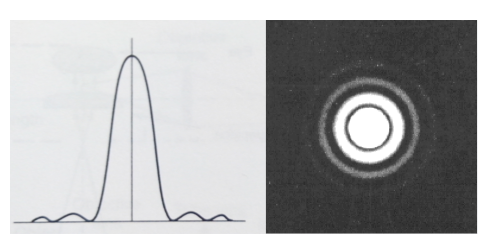
\includegraphics[width=0.7\textwidth]{capitulo2/airydisk}
\caption{Distribuci\'on de intensidad de un haz de luz y patr\'on de difracci\'on conocido como \emph{Airy Disk} \label{difra}}   %http://microscopy.berkeley.edu/courses/tlm/2P/index.html 
\end{figure}

A finales del siglo XIX el f\'isico Ernst Abbe, quien trabajaba en la fabrica de microscopios de Carl Zeiss demostr\'o que la potencia o alcance de la resoluci\'on espacial de un microscopio depende de la longitud de onda de la luz utilizada para formar la imagen y del \'angulo con que el objetivo colecta la luz o apertura angular; con esto Abbe defini\'o la  \emph{apertura num\'erica} del objetivo como:

\begin{equation}
NA= n sin(\Theta) \label{apnu}
\end{equation}

donde $\Theta$ es la mitad de la apertura angular del objetivo de microscopio y $n$ es el \'indice de refracci\'on del medio entre el objetivo y la muestra \cite{libro}. Entre m\'as grande sea el cono de luz que puede dirigirse a la lente m\'as grande ser\'a su apertura num\'erica. De la ecuaci\'on \ref{apnu} se puede ver que el m\'aximo valor que puede tomar la apertura num\'erica es el \'indice de refracci\'on; por lo que una manera de aumentar la apertura num\'erica es utilizar un medio de inmersi\'on con un \'indice de refracci\'on mayor que el aire, como puede ser el agua o aceite. N\'otese que el uso de objetivos de microscopio con apertura num\'erica grande, implica una disminuci\'on de la distancia entre la muestra y el objetivo. 

La resoluci\'on de un microscopio se define como la distancia $d$ entre dos part\'iculas adyacentes las cuales pueden ser percibidas como part\'iculas separadas. La resoluci\'on est\'a dada por el criterio Rayleigh:

\begin{equation}
d=\frac{1.22 \lambda}{2NA}
\end{equation}

donde $\lambda$ es la longitud de onda de la luz incidente en el vac\'io \cite{bioph}. De aqu\'i se  deduce que lentes con apertura \'optica mayor pueden brindar mejor resoluci\'on. 


El l\'imite de resoluci\'on por difracci\'on para un microscopio \'optico convencional, es decir, el detalle m\'as peque\~{n}o $\triangle x$ que puede ser resuelto con un microscopio en funci\'on de la longitud de onda $\lambda$ y apertura num\'erica $NA$ del objetivo es:

\begin{equation}
\triangle x=\frac{ \lambda}{2NA}
\end{equation}

Esta ecuaci\'on se conoce como la ecuaci\'on de Abbe \cite{libro}. La teor\'ia que desarrollo Abbe sobre el microscopio \'optico lo llevo a concluir que la resoluci\'on del microscopio est\'a determinada por la apertura num\'erica y no la magnificaci\'on; adem\'as concluy\'o que longitudes de onda m\'as cortas incrementan la resoluci\'on.

Otras distorsiones que se presentan en el sistema \'optico del microscopio e impiden la formaci\'on de una imagen perfecta se conocen como aberraciones. Hay dos tipos principales de aberraciones que desv\'ian la luz a causa de las propiedades de las lentes, o bien,  las formas geom\'etricas de las superficies reflejantes y de refracci\'on: aberraci\'on crom\'atica y esf\'erica. La primera se debe a la dependencia que tiene el \'inidce de refracci\'on con la longitud de onda, provocando que la luz se refracte con direcciones diferentes; mientras que la aberraci\'on esf\'erica se debe a la forma de las lentes, con distancias focales diferentes dependiendo de la zona de la lente.

El dise\~{n}o y manufactura de un microscopio buscan minimizar las aberraciones, maximizar la resoluci\'on y alcanzar la m\'axima fidelidad posible entre el objeto y la imagen con el contraste suficiente.  

El microscopio de fluorescencia ha emergido como una gran t\'ecnica para la adquisici\'on de im\'agenes de sistemas vivos; la fluorescencia proveniente de la muestra se utiliza para obtener la imagen. Se puede utilizar fluorescencia end\'ogena o se puede marcar el esp\'ecimen biol\'ogico con un fluor\'oforo, cuya distribuci\'on ser\'a evidente despu\'es de la iluminaci\'on. 

La microscopia de fluorescencia es idealmente utilizada para la detecci\'on de fluor\'oforos espec\'ificos en c\'elulas y tejidos. Se han desarrollado algunos microscopios cuyo funcionamiento se basa en la fluorescencia como el microscopio de epifluorescencia, confocal de barrido l\'aser y multifot\'on.


%%%%%%%%%% MICROSCOPIO DE epiFLUORESCENCIA %%%%%%%%%%%%%%%%%%%%%%%%%%%%%%%%%%%%  esp�cimen 

\subsection{Microscopio de epifluorescencia}\label{microscopito}


El microscopio m\'as utilizado hoy en d\'ia sigue el dise\~{n}o b\'asico de epifluorescencia. En este dispositivo la luz de excitaci\'on pasa a trav\'es del mismo objetivo de microscopio que posteriormente recolectar\'a la luz emitida por la muestra para formar la imagen; utilizando para ello filtros y un divisor de haz como se muestra en la figura \ref{epi}.

El divisor de haz transmite o refleja la luz dependiendo de su longitud de onda y separa la luz de excitaci\'on de la fluorescencia; la longitud de onda de la luz emitida es m\'as grande que la de excitaci\'on. En el sistema de iluminaci\'on se utilizan fuentes con un amplio rango espectral como l\'amparas de mercurio o xen\'on y con ayuda de un filtro se selecciona una longitud de onda espec\'ifica (com\'unmente en el rango UV). 

\begin{figure}[ht]
\centering
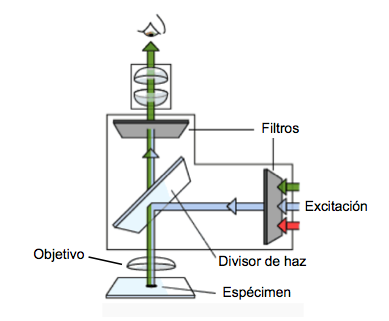
\includegraphics[width=3.2in, height=2.5in]{capitulo2/micrfluor}
\caption{Principio b\'asico de microscopio de epifluorescencia. \emph{\scriptsize{Imagen obtenida de http://www.nobelprize.org/educational/physics/microscopes/fluorescence/, sin datos de autor.}} \label{epi}}   
\end{figure}

Este tipo de microscopio tiene varias ventajas: el objetivo (utilizado primero para concentrar y enfocar la luz incidente en la muestra y despu\'es como colector de la luz emitida para formar la imagen) siempre est\'a en correcta alineaci\'on; la mayor parte de la luz de excitaci\'on atraviesa el esp\'ecimen y se aleja del objetivo; la zona iluminada de la muestra se limita a lo que puede ser observado; se puede utilizar la apertura num\'erica completa del objetivo de microscopio; es posible combinar o alternar la manera de obtener la imagen, analizando la fluorescencia de la muestra o la luz transmitida \cite{ventajasepi}.


%%%%%%%%%%%%%%%%%%%%%%%%%%%%%%microscopia confocal de barrido laser
\subsection{Microscop\'ia confocal de barrido l\'aser}

La microscop\'ia confocal es una t\'ecnica que puede aumentar la resoluci\'on y el contraste de una imagen con el uso de una iluminaci\'on puntual y una abertura confocal en el camino del haz que forma la imagen (fluorescencia en el caso del microscopio de fluorescencia). El objetivo de la apertura, que puede ser un pinhole, es eliminar las contribuciones de la luz fuera de foco como se explica en el esquema de la figura \ref{confo}. 

\begin{figure}[ht]
\centering
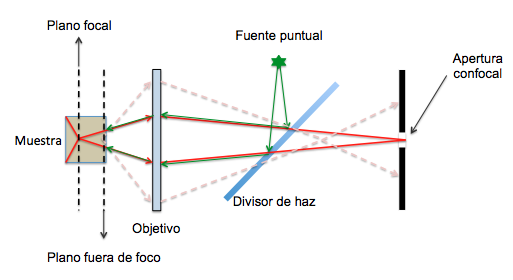
\includegraphics[width=0.95\textwidth]{capitulo2/confocal2}
\caption{\small{Trayectoria de la luz en un microscopio confocal de fluorescencia. La luz fuera del plano focal no es detectada debido a la apertura confocal.}\label{confo}}   
\end{figure}

La t\'ecnica que combina la microscop\'ia confocal y de fluorescencia es la microscop\'ia confocal de barrido l\'aser, en donde la fuente de excitaci\'on es un haz l\'aser enfocado por un objetivo a la muestra. La extensi\'on espacial del l\'aser enfocado en la muestra es determinado por la longitud de onda, la apertura num\'erica de las lentes y la calidad de formaci\'on de la imagen. 

La principal caracter\'istica de esta t\'ecnica es la capacidad de adquirir im\'agenes a profundidades espec\'ificas del tejido (de hasta 100 micrometros) permitiendo reconstrucciones en 3D. Otra ventaja de este dispositivo es que la magnificaci\'on puede ajustarse variando el \'area de barrido del l\'aser en la muestra sin necesidad de cambiar los objetivos, esta caracter\'istica se conoce como \emph{zoom factor} \cite{lscm}.

La fluorescencia utilizada para formar la imagen en este microscopio es inducida por la absorci\'on de un fot\'on y es un proceso lineal, por ello la fluorescencia se manifiesta a lo largo de un cono de luz como se observa en la imagen izquierda de la figura \ref{puntual}; esto puede provocar da\~{n}o fotoqu\'imico en un \'area grande de la muestra.

La mayor\'ia de fluor\'oforos utilizados en esta t\'ecnica, como marcadores en sistemas vivos son excitados por la absorci\'on de un fot\'on en la regi\'on UV o azul de la luz. A esta longitud de onda la luz es altamente atenuada por el tejido y limita la adquisici\'on de im\'agenes con gran profundidad de penetraci\'on \cite{bioph}.

\begin{figure}
\centering
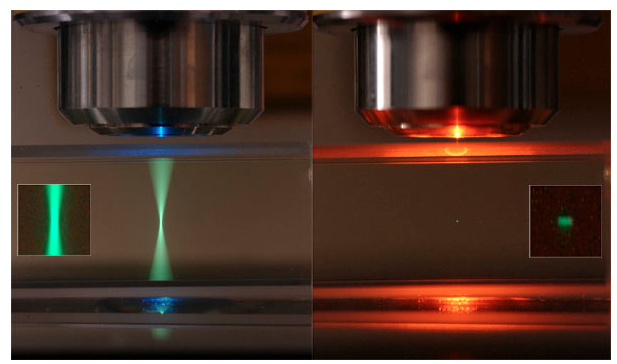
\includegraphics[width=0.7\textwidth]{capitulo2/compara}
\caption{Haz de excitaci\'on para microscop\'ia de barrido l\'aser de uno y dos fotones. \emph{\scriptsize{Imagen de  Steve Ruzin y Holly Aaron, UC Berkeley.}}\label{puntual}}   %http://microscopy.berkeley.edu/courses/
\end{figure}

%%%%%%%%%% MICROSCOPIO multifot�n %%%%%%%%%%%%%%%%%%%%%%%%%%%%%%%%%%%%  esp�cimen 
\subsection{Microscop\'ia multifot\'on}

En la microscop\'ia multifot\'on un fluor\'oforo es excitado mediante la absorci\'on de dos o mas fotones y la fluorescencia emitida se usa para formar una imagen. La fluorescencia inducida por la absorci\'on de dos o tres fotones se ha utilizado en este tipo de microscop\'ia no lineal. Sin embargo, por razones pr\'acticas (luz de excitaci\'on de gran intensidad) que requiere el proceso de absorci\'on de tres fotones, solo la microscop\'ia de dos fotones ha emergido como una de las t\'ecnicas m\'as utilizadas para adquisici\'on de im\'agenes de sistemas vivos. 

La absorci\'on de dos fotones es un fen\'omeno no lineal que fue propuesto te\'oricamente por Maria G\"{o}ppert- Mayer. En este proceso un \'atomo tiene una transici\'on del estado base $S_{0}$ al estado excitado $S_{n}$ por la absorci\'on "simult\'anea" de dos fotones (Ver Figura \ref{diagramatpa}); el primer fot\'on induce la trasici\'on del estado base a un estado virtual y el segundo fot\'on induce la transici\'on del estado virtual al estado excitado. 

\begin{figure}
\centering
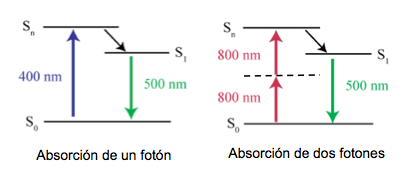
\includegraphics[width=4.2in, height=2.2in]{capitulo2/tpa1}
\caption{Diagrama de energ\'ia para la transici\'on de uno y dos fotones. \emph{\scriptsize{Imagen de D. Nowak}} 
 \label{diagramatpa}}    
\end{figure}

La probabilidad del proceso de absorci\'on de dos fotones depende de la intensidad de la luz de excitaci\'on elevada al cuadrado, por eso es necesario el uso de un l\'aser con pulsos intensos. La microscop\'ia de barrido l\'aser de dos fotones puede utilizar un l\'aser enfocado de pulsos cortos (del orden de picosegundos y femtosegundos) con longitud de onda en el rojo o cercano infrarrojo  como fuente de excitaci\'on y puede producir fluorescencia en el rango visible. 

El uso de un haz de excitaci\'on enfocado en esta t\'ecnica de microscop\'ia presenta ventajas como la implementaci\'on de resoluci\'on espacial sin el uso de \emph{pinholes}  o rendijas como filtros espaciales, la obtenci\'on de im\'agenes 3D y la confinaci\'on de la destrucci\'on fotoqu\'imica al volumen focal como se muestra en el lado derecho de la figura \ref{puntual}). Adem\'as como las c\'elulas y tejidos presentan relativa transparencia ante la radiaci\'on infrarroja (Ver Figura \ref{penetrad}), la microscop\'ia de barrido l\'aser de dos fotones aumenta la profundidad de penetraci\'on en espec\'imenes vivos; mientras m\'as grande sea la longitud de onda de la luz de excitaci\'on, el da\~{n}o a las c\'elulas y tejidos es menor.

Esta t\'ecnica es ideal para adquirir im\'agenes de diversas profundidades en tejidos, con una resoluci\'on de submicr\'ometros: $0.3\mu m$ de resoluci\'on lateral, $0.8\mu m$ de resoluci\'on axial y una profundidad de penetraci\'on que puede ir de $500$ a $1000\mu m$ \cite{libro}.

%En la pr\'actica la resoluci\'on espacial del microscopio de absorci\'on de dos fotones es similar al microscopio confocal de fluorescencia. El primero tiene una resoluci\'on ligeramente menor en comparaci\'on con el microscopio confocal pero el uso de una abertura confocal provoca p\'erdidas en la se\~{n}al.

\begin{figure}
\centering
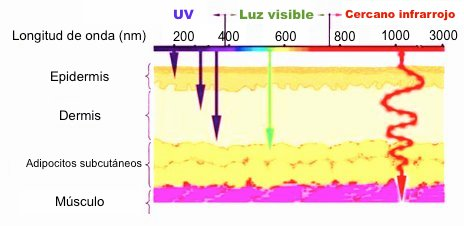
\includegraphics[width=4.5in, height=2.2in]{capitulo2/penetrasyo}
\caption{Esquema de penetraci\'on del tejido a diferentes longitudes de onda. \emph{\scriptsize{Imagen tomada del art�culo "The Impact of Near-infrared in Plastic Surgery", Ibima Publishing.}} \label{penetrad}}    
\end{figure}

\section{Propiedades \'opticas de marcadores en microscopia de fluorescencia}

Hay diversos materiales org\'anicos e inorg\'anicos que presentan una gran emisi\'on de luz y se utilizan como marcadores biocompatibles en microscop\'ia de fluorescencia. El estudio \'optico lineal y no lineal de estos materiales, desde colorantes comerciales hasta nanopart\'iculas de nuevos compuestos, incluye por ejemplo el an\'alisis de propiedades como la eficiencia cu\'antica de fluorescencia o la secci\'on transversal de absorci\'on de dos fotones, la cual es relevante para los marcadores en microscop\'ia de barrido l\'aser de dos fotones.

Por otra parte, un fen\'omeno que ha sido \'util en la microscop\'ia de fluorescencia, es la Transferencia de Energ\'ia de Resonancia F\"orster \'o FRET por sus siglas en ingl\'es. Esta transferencia de energ\'ia permite modificar algunas  propiedades \'opticas de un fluor\'oforo utilizando otro compuesto o colorante bajo ciertas condiciones mostradas m\'as adelante.  
  
\subsection{Eficiencia cu\'antica de fluorescencia}

Los procesos de decaimiento que llevan a una mol\'ecula  del estado excitado al estado base pueden ser radiativos y no radiativos. Como decaimientos no radiativos se pueden citar la conversi\'on interna y transiciones entre dos estados el\'ectronicos (que pueden llevar a la emisi\'on de fosforescencia) entre otros; sin embargo, el proceso de decaimiento predominante en el tipo de materiales que se estudiaron en este trabajo es radiativo: la fluorescencia; que es un tipo de luminiscencia con una tasa de emisi\'on de $10^{8} s^{-1}$ y un tiempo de vida de varios nanosegundos. 

%La luminiscencia puede ser fosforescencia o fluorescencia, dependiendo de la naturaleza del estado excitado. La tasa de emisi\'on de la fosforescencia es de $10^{3}$ a $1 s^{-1}$ y tiene un tiempo de vida del orden de milisegundos; sin embargo, la tasa de emisi\'on de la fluorescencia es t\'ipicamente del orden de  y tiene un tiempo de vida de varios nanosegundos .

La eficiencia cu\'antica de fluorescencia $\Phi_{f}$ es la raz\'on que hay entre los fotones absorbidos por un compuesto y los emitidos mediante fluorescencia como se muestra en la ecuaci\'on \ref{eficuan}. La eficiencia cu\'antica de fluorescencia, determina la probabilidad de que una mol\'ecula en estado excitado tenga un decaimiento radiativo por fluorescencia, en lugar de cualquier otro mecanismo no radiativo \cite{UK}.

\begin{equation}
\Phi_{f}=\frac{\# fotones \hspace{0.2cm} emitidos}{\# fotones  \hspace{0.2cm} absorbidos} \label{eficuan}
\end{equation}

Desde hace algunas d\'ecadas, se han realizado esfuerzos para desarrollar m\'etodos confiables que determinen la eficiencia cu\'antica de fluorescencia, la mayor\'ia de los cuales utilizan el compuesto de inter\'es en soluci\'on o suspensi\'on.

Los m\'etodos que buscan determinar directamente la eficiencia cu\'antica de fluorescencia, se conocen como m\'etodos absolutos. Por ejemplo el m\'etodo Vavilov, monitorea la fluorescencia de la muestra en una celda y el esparcimiento de una superficie s\'olida de \'oxido de magnesio; en el m\'etodo de Weber y Teale, a diferencia del anterior, se analiza el esparcimiento de una soluci\'on y el m\'etodo calor\'imetrico, mide la energ\'ia liberada en forma de calor por los decaimientos no radiativos. 

Debido a las complejas correcciones que requieren diversos m\'etodos absolutos, en la gran mayor\'ia de laboratorios se utiliza el m\'etodo relativo para medir $\Phi_{f}$. Este m\'etodo se basa en comparar la intensidad de fluorescencia de la muestra de inter\'es con la intensidad de fluorescencia de una soluci\'on de referencia \cite{tesisdoc}. En particular, en este trabajo se midi\'o la eficiencia cu\'antica de fluorescencia con un m\'etodo relativo utilizando una esfera integradora.

\subsubsection{M\'etodo relativo de la esfera integradora para medir eficiencia cu\'antica de fluorescencia}

En este m\'etodo se mide la eficiencia cu\'antica de fluorescencia $ \Phi_f$ para un compuesto en soluci\'on o suspensi\'on de nanopart\'iculas mediante la detecci\'on de emisi\'on de luz de \'este en una esfera integradora; para ello se utiliza un sistema de detecci\'on, que puede ser constituido por un monocromador, una c\'amara CCD, un analizador multicanal fot\'onico, un fotodetector etc... Particularmente, en este trabajo se utiliz\'o un un tubo fotomultiplicador o PMT por sus siglas en ingles y un amplificador lock- in. 

Las soluciones o suspensiones se colocan en celdas de cuarzo de $0.1\times1\times4 cm^{3}$ a concentraciones del orden de $10^{-6}$ y $10^{-7}$ M. La emisi\'on de luz de la muestra es reflejada con la misma intensidad en todas direcciones dentro de la esfera integradora y detectada por un PMT colocado en una abertura de la esfera. El PMT, detecta los fotones de emisi\'on y crea una se\~{n}al el\'ectrica que es enviada a un amplificador lock- in. Finalmente el amplificador arroja el valor, en volts, de la se\~{n}al causada por la intensidad de fluorescencia.

El proceso anterior se repite para una soluci\'on utilizada como referencia con valor de eficiencia cu\'antica de fluorescencia conocido. Comparando la emisi\'on de luz de la muestra de inter\'es con la emisi\'on de luz de la referencia se puede conocer $\Phi_f$ para la muestra, como se explica a continuaci\'on. 

Cuando el haz de excitaci\'on incide en un medio, en este caso la celda, parte de la luz ser\'a transmitida, reflejada y absorbida por el medio. La aplicaci\'on de la conservaci\'on de energ\'ia, determina que la suma de la transmisi\'on $t$ , reflexi\'on $r$ y absorci\'on $a$ de la luz incidente es igual a la unidad.

\begin{equation}
t+r+a=1  \label{1}
\end{equation}  

En el m\'etodo utilizado en este trabajo, el reflejo del haz de excitaci\'on en la celda se dirigi\'o hacia afuera de la esfera integradora para no ser detectado y as\'i suponer que $r=0$ en la ecuaci\'on \ref{1}. %%%no es cierto en la realidad la luz reflejada es distinta de cero pero su contribuci�n se elimina utilizando tambi�n la referencia!!!!

La intensidad de la luz emitida por una muestra $I_m$ es proporcional a la intensidad de luz del haz incidente $I_{0 _m}$, eficiencia cu\'antica de fluorescencia $\Phi_{f_m}$ y absorci\'on $a$; esta \'ultima se puede expresar como $a=1-t$ para escribir:

\begin{equation}
I_{m}\propto I_{0m} \Phi_{f_m}(1-t) \label{prop}
\end{equation}  

N\'otese que se ha utilizado el sub\'indice $m$ para hacer referencia a los par\'ametros de la muestra de inter\'es. Utilizando la Ley de Lambert- Beer es posible expresar la transmisi\'on como $t=10^{-A_{m}}$, donde $A_{m}$ es la absorbancia de la muestra. La ecuaci\'on \ref{prop} puede escribirse como 

\begin{equation}
I_{m}=k I_{0m} \Phi_{m}(1-10^{-A_{m}}) \label{igual}
\end{equation}  
 
donde se introdujo la constante instrumental $k$. El valor de esta constante de correcci\'on para el sistema completo de medici\'on de eficiencia cu\'antica no es conocido, pero puede ser eliminado de la ecuaci\'on \ref{igual} utilizando una soluci\'on de prueba o referencia con valor de eficiencia cu\'antica de fluorescencia conocido. Es decir, la intensidad de emisi\'on de la muestra de referencia $I_{ref}$ es  $I_{ref}=k I_{0 ref} \Phi_{f_{ref}}(1-10^{-A_{ref}})$, donde se especifica que se trata de la referencia con el sub\'indice $ref$. 

En los experimentos realizados en este trabajo, se midi\'o la intensidad de fluorescencia de la muestra de inter\'es y de la referencia bajo las mismas condiciones y se utiliz\'o la misma intensidad de excitaci\'on\footnote{No es una condici\'on necesaria cuando el sistema de detecci\'on responde de manera lineal para distintos valores de intensidades incidentes de inter\'es}, es decir, $I_{0m}=I_{0 ref}$. Bajo estas circunstancias, resolviendo el sistema de ecuaciones para $\Phi_{f_m}$ se tiene que: 

\begin{equation}
\Phi_{f_m}= \Phi_{f_{ref}} \frac{I_{m}}{I_{ref}} \frac{(1-10^{-A_{ref}})}{(1-10^{-A_{m}})}  \label{final}
\end{equation}  
 
$ \Phi_{f_{ref}}$ es el valor conocido de la eficiencia cu\'antica de fluorescencia para la referencia. En este experimento $I_{m}$ e $I_{ref}$ son par\'ametros referentes a la detecci\'on del nivel de intensidad de emisi\'on de la muestra y de la referencia, cuyos valores (al ser detectados con un PMT) est\'an dados en volts; los valores de absorbancia para la muestra y la referencia a la misma longitud de onda que el haz de excitaci\'on se conocen con los espectros de absorci\'on, los cuales se adquieren en celdas de cuarzo con la misma longitud de camino \'optico y la misma concentraci\'on molar que se utilizaron en este m\'etodo.
 
  
%Essentially, solutions of the standard and test samples with identical absorbance at the same excitation wavelength can be assumed to be absorbing the same number of photons.

\subsection{Procesos no lineales: Absorci\'on de dos fotones}

La \'optica no lineal estudia los fen\'omenos que ocurren como consecuencia de la modificaci\'on de las propiedades \'opticas de un material por la presencia de luz, t\'ipicamente luz l\'aser. Los fen\'omenos \'opticos son no lineales, porque ocurren cuando la respuesta de un material al campo \'optico aplicado depende de una manera no lineal de la amplitud de dicho campo \'optico \cite{boyd}.

Para comprender lo anterior es importante analizar la dependencia que tiene la polarizaci\'on de un material con la amplitud del campo el\'ectrico aplicado. En la \'optica convencional o lineal, la polarizaci\'on inducida depende linealmente de la amplitud del campo el\'ectrico; sin embargo, en \'optica no lineal la respuesta se generaliza expresando la polarizaci\'on inducida $P(t)$ como sigue:
 
\begin{equation}
\label{que}
P(t)=\epsilon_{0}[\chi^{(1)}E(t)+\chi^{(2)} E^2(t)+\chi^{(3)} E^{3}(t)+...]
\end{equation}

donde $\epsilon_{0}$ es la permitividad en el vac\'io y $\chi^{(1)}$, $\chi^{(2)}$ y  $\chi^{(3)}$ representan la susceptibilidad el\'ectrica de primero, segundo y tercer orden respectivamente. Por simplicidad, en la ecuaci\'on anterior \'unicamente se toma en cuenta el car\'acter escalar tanto de la polarizaci\'on como del campo el\'ectrico y se asume una polarizaci\'on instant\'anea y por lo tanto una susceptibilidad el\'ectrica constante (no hay p\'erdidas ni dispersi\'on). 

La polarizaci\'on juega un papel importante en la descripci\'on de fen\'omenos no lineales porque cuando var\'ia en el tiempo, puede actuar como fuente de nuevos componentes del campo electromagn\'etico.

La absorci\'on de dos fotones es una consecuencia de la polarizaci\'on no lineal de tercer orden, dicha polarizaci\'on se puede identificar de la ecuaci\'on \ref{que} como $P^{(3)}(t)=\epsilon_{0}\chi^{(3)} E^{3}(t)$. Si se considera un campo el\'ectrico monocrom\'atico de la forma $E(t)=\xi cos(wt)$, incidiendo en un material tal que $\chi^{(3)}\neq0$ \footnote{La susceptibilidad el\'ectrica de tercer orden es diferente de cero sin importar el material, puede ser un medio centrosim\'etrico o no centrosim\'etrico.}, la polarizaci\'on no lineal de tercer orden se expresa como:

\begin{equation}
\label{que2}
P^{(3)}(t)=\frac{1}{4}\epsilon_{0}\chi^{(3)}\xi^{3} cos(3wt)+\frac{3}{4}\epsilon_{0}\chi^{(3)}\xi^{3} cos(wt) 
\end{equation}

donde se utiliz\'o la identidad trigonom\'etrica $cos^{3}(w)= \frac{1}{4} cos(3wt)+\frac{3}{4} cos(wt)$. El primer t\'ermino de la ecuaci\'on \ref{que2} describe una respuesta de frecuencia $3w$ creada por un campo incidente de frecuencia $w$, este proceso se conoce como generaci\'on de tercer arm\'onico o THG por sus siglas en ingl\'es. 

El segundo t\'ermino de la ecuaci\'on \ref{que2} describe la contribuci\'on no lineal de la polarizaci\'on a la misma frecuencia que el campo incidente; este t\'ermino, como se explica m\'as adelante, es la contribuci\'on no lineal al \'indice de refracci\'on que experimenta una onda de frecuencia $w$. En la figura \ref{dibujo3o} se muestra un medio no lineal en el que incide un campo de frecuencia $w$, la polarizaci\'on no lineal de tercer orden creada en este medio tiene contribuciones de frecuencias $w$ y $3w$.

\begin{figure}[ht]
\centering
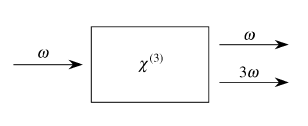
\includegraphics[width=0.6\textwidth]{capitulo2/tercerorden}
\caption{Geometr\'ia del efecto de la polarizaci\'on no lineal de tercer orden \label{dibujo3o}}   
\end{figure}

De manera general, el estudio de la polarizaci\'on no lineal de tercer orden se desarrolla considerando un campo el\'ectrico incidente compuesto por  tres frecuencias no necesariamente iguales, por lo que habr\'a diversas  contribuciones a la polarizaci\'on no lineal correspondientes a las frecuencias resultantes de la combinaci\'on de las frecuencias incidentes (Generaci\'on de terceros arm\'onicos, diferencia y suma de frecuencias y las mismas frecuencias incidentes).  

Para visualizar lo anterior, consid\'erese un campo el\'ectrico polarizado en la direcci\'on $i$ incidiendo en un material no lineal; si se toma en cuenta que la polarizaci\'on no es instant\'anea, la polzarizaci\'on no lineal de tercer orden en el dominio de la frecuencia se escribe como:
 
\begin{equation}
P_i^{(3)}(\vec{r},w_4)=\triangle \epsilon_0 \chi^{(3)}_{ijkl}(-w_4;w_1,w_2,w_3)E_j(\vec{r},w_1)E_k(\vec{r},w_2) E_l(\vec{r},w_3) \label{wt}
\end{equation}   

donde $ \chi^{(3)}_{ijkl}$ es el tensor de susceptibilidad de tercer orden\footnote{N\'otese que el tensor de susceptibilidad el\'ectrica de tercer orden es un tensor de cuarto grado (En tres dimensiones tiene 81 componentes)} y se cumple la relaci\'on $w_4=w_1+w_2+w_3$.  El s\'imbolo $\triangle$ toma los valores de $1$ cuando $w_1=w_2=w_3$, $\triangle = 3$ cuando dos de las frecuencias son iguales y $\triangle=6$ si todas las frecuencias son diferentes.

Si se considera un campo incidente de frecuencia $w$ y se analiza la contribuci\'on a la polarizaci\'on no lineal de tercer orden correspondiente a la misma frecuencia incidente $w$, la ecuaci\'on \ref{wt} se expresa de la siguiente manera:

\begin{equation}
P_i^{(3)}(\vec{r},w)=3  \epsilon_0 \chi^{(3)}_{ijkl}(-w;w,w,-w)E_j(\vec{r},w)E_k(\vec{r},w) E^{\ast}_l(\vec{r},w)
\end{equation}

donde $E^{\ast}_l(\vec{r},w)=E_l(\vec{r},-w)$. Si el material es isotr\'opico, es decir, sus propiedades son las mismas en todas direcciones y asumimos que $i=j=k$, entonces debe observarse que $i=j=k=l$ y la expresi\'on anterior se escribe como $P^{(3)}(\vec{r},w)=3  \epsilon_0 \chi^{(3)}(-w;w,w,-w)E(\vec{r},w) |E (\vec{r},w)|^2$. As\'i la polarizaci\'on total $P_T(\vec{r},w)$ para este caso en el que hay un campo incidente de frecuencia $w$ se escribe como:

\begin{align}
P_T(\vec{r},w)=\epsilon_0[ \chi^{(1)}+ 3 \chi^{(3)} |E(\vec{r},w)|^2] E(\vec{r},w)\label{pt} 
\end{align}

La polarizaci\'on de segundo orden es cero porque $\chi^{(2)} \neq 0$ \'unicamente en medios no centrosim\'etricos.

Por otro lado, la ecuaci\'on de onda en el dominio de la frecuencia $\Omega$ se expresa como $\nabla^2\vec{E}(\vec{r},\Omega)+\frac{\Omega^2}{c^2}\vec{E}(\vec{r},\Omega)=-\mu_{0}\Omega^2\vec{P}(\vec{r},\Omega)$,donde $\mu_{0}=\frac{1}{c^{2} \epsilon_{0}}$ es la constate magn\'etica en el vac\'io.

Si en la polarizaci\'on total de la ecuaci\'on \ref{pt} se considera un campo el\'ectrico polarizado en direcci\'on $i$, cuya direcci\'on de propagaci\'on est\'a en la direcci\'on $z$ ($\vec{r}=z\hat{k}$), entonces la ecuaci\'on de onda en el dominio de la frecuencia se escribe como:

\begin{align}
\frac{\partial^2}{\partial z^2}E_{i}(z,w)+\left[\frac{w}{c}\right]^2 E_{i}(z,w)=-\frac{w^2}{c^2}[\chi^{(1)}_{ii}E_{i}(z,w)+\chi^{(3)}_{iiii}|E(z,w)|^2 E_{i}(z,w)]
\end{align}
 
Proponiendo la soluci\'on $E_{i}(z,w)=\xi(z)e^{ikz}$ y utilizando la Aproximaci\'on de Envolvente de Variaci\'on Lenta\footnote{En esta aproximaci\'on la amplitud $\xi(z)$ varia muy lentamente por lo que $\frac{d\xi_{i}(z)}{dz}\gg \frac{d^2\xi_{i}(z)}{dz^2}$} (SVEA) se tiene que:

\begin{align}
\frac{d\xi(z)}{\xi(z)}=\frac{3i}{2k}\left[\frac{w}{c}\right]^2 \chi^{(3)}_{iiii} |\xi(z)|^2 dz\label{svea}
\end{align}

en donde $(1+\chi^{(1)}_{ii})(w^2/c^2)=k^2$. 

Si se asume que que $\chi^{(3)}_{iiii}$ es real y se integra la ecuaci\'on \ref{svea} se obtiene como soluci\'on $E(z,w)=\xi_0 e^{i\{ \frac{w}{c}n+  \frac{3}{2}\frac{w}{c}\frac{1}{n} \chi^{(3)}_{iiii} |\xi_0|^2\}z}$ donde se utiliz\'o que $k=\frac{w}{c}n$. En analog\'ia con el r\'egimen lineal se puede apreciar que el \'indice de refracci\'on total $n_T$ , ahora tiene la contribuci\'on no lineal  $\frac{3}{2}\frac{1}{n} \chi^{(3)}_{iiii} |\xi_0|^2$; por lo que en t\'erminos de intensidad se tiene que el \'indice de refracci\'on total $n_T$ es:

\begin{align}
n_T=n+  n_2 I
\end{align}

donde $n_2=\frac{3\chi^{(3)}_{iiii}}{\epsilon_0 n^2c}$ es el \'indice de refracci\'on no lineal de intensidad conocido como coeficiente Kerr y la intensidad es $I=\frac{1}{2}n\epsilon_0 c  |\xi(z)|^2$. %Esto indica que en el r\'egimen no lineal el \'indice de refracci\'on depende de la intensidad.

Sin embargo, el tensor de susceptibilidad el\'ectrica de tercer orden tiene tambi\'en una parte imaginaria. Para conocer el efecto de absorci\'on se asume ahora que $\chi^{(3)}_{real}=0$, por lo que sustituyendo $\chi^{(3)}=i \chi^{(3)}_{im}$ en la ecuaci\'on \ref{svea} se obtiene $\frac{d|\xi(z)|^2}{dz}=-\beta_E|\xi(z)|^4$, donde se ha definido $\beta_E=\frac{3w\chi^{(3)}_{im}}{cn}$ como el coeficiente de absorci\'on no lineal referente al capo el\'ectrico. Y en t\'erminos de la intensidad: 

\begin{align}
\frac{dI}{dz}=-\beta I^2 \label{porfin}
\end{align}

donde $\beta=\frac{6w\chi^{(3)}_{im}}{c^2n_f^2 \epsilon_0}$ es el coeficiente de absorci\'on no lineal referente a la intensidad. As\'i, tanto el coeficiente de refracci\'on $n_2$ como el coeficiente de absorci\'on $\beta$ no lineales dependen de la intensidad.

Tomando en cuenta la absorci\'on lineal mediante la Ley de Lambert- Beer la ecuaci\'on \ref{porfin} se escribe como:

\begin{align}
\frac{dI}{dz}=-\alpha I  -\beta I^2=-\alpha_T I
\end{align}

donde $\alpha$ es el coeficiente de absorci\'on lineal y $\alpha_T (I)=\alpha+\beta I$ es el coeficiente de absorci\'on efectivo del material. La soluci\'on de esta ecuaci\'on diferencial es: $I(z)=\frac{\alpha e^{-\alpha z}}{1-\beta e^{-\alpha z}}$, lo cual da lugar a dos tipos de absorci\'on dependiendo del signo de $\beta$.  

Si $\beta<0$ el coeficiente de absorci\'on efectivo disminuye cuando la intensidad crece, esto se conoce como absorci\'on saturable. Esta absorci\'on vuelve a los materiales transparentes a medida que la intensidad del campo el\'ectrico incidente aumenta.


Sin embargo, cuando $\beta>0$ el coeficiente de absorci\'on efectivo aumenta con la intensidad como se muestra en la figura \ref{grafiquita}. Este proceso se conoce como absorci\'on de dos fotones; fue descrito por primera vez, de forma te\'orica por Maria Goppert- Mayer en 1931 \cite{megalibro} y observado experimentalmente por Kaiser y Garret en 1961 \cite{boyd}.

\begin{figure}[ht]
\centering
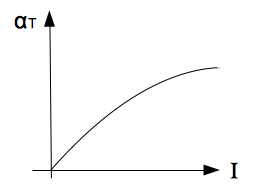
\includegraphics[width=0.34\textwidth]{capitulo2/gra2}
\caption{Absorci\'on de dos fotones \label{grafiquita}}   
\end{figure}

En este proceso, un \'atomo hace una transici\'on del estado base a un estado excitado mediante la absorci\'on \emph{simult\'anea} de dos fotones como se muestra en la figura \ref{diagramatpa}. Se dice que este proceso es simult\'aneo porque dos fotones deben interactuar en un estado virtual en un tiempo $\tau$ de $10^{-15}$ o $10^{-16}s$ para que se de la absorci\'on y el \'atomo sea promovido al estado excitado \cite{todoTPA}. La probabilidad de absorci\'on de dos fotones es proporcional al cuadrado de la intensidad de excitaci\'on. 

%Una aplicaci\'on basada en los efectos de la absorci\'on de dos fotones es un limitador \'optico que no permite el paso de luz si la intensidad es grande, evitando as\'i posibles da\~{n}os en circuitos \'opticos.


El efecto de absorci\'on de dos fotones se puede cuantificar introduciendo un par\'ametro conocido como secci\'on transversal de absorci\'on de dos fotones $\sigma^{TPA}$, el cual determina la magnitud del mismo proceso de absorci\'on. 

De la misma manera que la secci\'on transversal de absorci\'on lineal est\'a relacionada con el coeficiente de absorci\'on lineal, la relaci\'on entre $\beta$ y $\sigma^{TPA}$ es:

\begin{align}
\beta=N_g \frac{\sigma^{TPA}}{\hbar w}
\end{align}

donde $N_g$ es el n\'umero de mol\'eculas por volumen en el estado base. As\'i la ecuaci\'on \ref{porfin} se puede escribir de la siguiente manera:

\begin{align}
\frac{dI}{dz}= -N_g \sigma^{*TPA} I^2= -N_g \frac{\sigma^{TPA}}{\hbar w} I^2
\end{align}

donde $\sigma^{*TPA}$ es un coeficiente relacionado con la absorci\'on de dos fotones \cite{rescatetpa}. Las unidades de la secci\'on transversal de absorci\'on de dos fotones $\sigma^{TPA}$ son los G\"oppert- Mayer o [GM] (1GM=$10^{-50} cm^4 s fot\'on^{-1} mol\'ecula^{-1}$) mientras que las unidades de $\sigma^{*TPA}$ son [$longitud^4  mol\'ecula^{-1} potencia^{-1}$].

En t\'erminos del flujo de fotones $f$ teniendo en cuenta que $f=I/\hbar w$ la ecuaci\'on anterior se expresa como: $\frac{df}{dz}= -N_g \sigma^{TPA} f^2 \label{flujo}$. Sin embargo, el t\'ermino $df/dz$ representa la velocidad de atenuaci\'on por la absorci\'on de dos fotones a lo largo de la direcci\'on de propagaci\'on; esto significa que el n\'umero de fotones absorbidos $N(t)$ por unidad de tiempo y volumen es:
 
\begin{align}
N(t)= -\frac{df}{dz}=N_g \frac{\sigma^{TPA}}{(\hbar w)^2} I^2=\frac{\beta I^2}{\hbar w}
\end{align}


Hay diversas t\'ecnicas experimentales para determinar $\sigma^{TPA}$ o bien $\beta$, pueden ser t\'ecnicas directas, indirectas y de mezcla de ondas.

Los m\'etodos directos se basan en medir la atenuaci\'on de un haz l\'aser al atravesar el medio absorbedor; en los m\'etodos indirectos se mide uno de los efectos inducidos por la absorci\'on de dos fotones y en el mezclado de ondas se utiliza m\'as de un haz, com\'unmente incidiendo en direcciones diferentes en el medio.


\subsection{Medici\'on de $\sigma^{TPA}$ mediante la t\'ecnica de TPEF}

Un material que presenta una absorci\'on de dos fotones pasa del estado base al estado electr\'onico excitado. Despu\'es de un relajamiento inicial no radiativo, la energ\'ia de excitaci\'on restante se libera mediante uno o m\'as procesos f\'isicos; los m\'etodos indirectos que determinan $\sigma^{TPA}$ monitorean uno de los posibles procesos de de- excitaci\'on que llevan al \'atomo al estado base.

La t\'ecnica indirecta m\'as com\'un, utilizada en este trabajo, se denomina t\'ecnica de emisi\'on inducida por absorci\'on de dos fotones (TPEF por sus siglas en ingl\'es). En esta t\'ecnica se utiliza un haz l\'aser de gran intensidad, generalmente pulsado y enfocado para concentrar la energ\'ia en la muestra, y se mide la se\~{n}al de fluorescencia generada por la absorci\'on de dos fotones; de esta se\~{n}al de fluorescencia se puede determinar la secci\'on transversal de excitaci\'on de dos fotones $\sigma^{TPE}$, la cual es linealmente proporcional a la secci\'on transversal de absorci\'on de dos fotones $\sigma^{TPA}$ \cite{pre_rigo}, o bien:

\begin{align}
\sigma^{TPE}=\Phi_f \sigma^{TPA}
\end{align}

Como se vio en la secci\'on anterior el n\'umero de fotones absorbidos $N(t)$ por mol\'ecula, por unidad de tiempo es proporcional a la secci\'on transversal de absorci\'on de dos fotones y del cuadrado de la intensidad incidente. Sin embargo en un experimento particular, el n\'umero total de fotones absorbidos $N_{abs}(t)$ est\'a en funci\'on tambi\'en de la concentraci\'on $c$ de la muestra y del volumen $V$ iluminado en la misma \cite{maso}:

\begin{align}
N_{abs}(t)=\int_V \sigma^{TPA} c I^2(\vec{r},t)dV
\end{align}

Adem\'as se suele separar la dependencia temporal y espacial de la intensidad de excitaci\'on, es decir, $I^2(\vec{r},t)=S(\vec{r})I_0(t)$. Por lo que lo anterior se escribe como:

\begin{align}
 N_{abs}(t)= \sigma^{TPA} c I_0^2(t)\int_V  S^2(\vec{r})dV \label{k}
\end{align}

Por otra parte, el n\'umero total de fotones absorbidos por unidad de tiempo $N_{abs}(t)$ en un proceso de absorci\'on de dos fotones, est\'a relacionado con el n\'umero de fotones de fluorescencia $F(t)$ detectados en el experimento de la siguiente manera: $F(t)=\frac{1}{2}\eta \Phi_f N_{abs}(t)$, donde $\eta$ es la eficiencia de colecci\'on de fluorescencia del sistema experimental. N\'otese que el factor de $1/2$ refleja el hecho de que dos fotones son necesarios en cada evento de excitaci\'on.

Sin embargo, en la pr\'actica solo el promedio temporal del flujo de fotones emitidos $\langle F(t)\rangle$ es medido, es decir: 

\begin{align}
\langle F(t)\rangle=\frac{1}{2} \eta \Phi_f c \sigma^{TPA} \langle I_0^2(t)\rangle \int_V dV S^2(\vec{r})
\end{align}

donde se utiliz\'o el valor de $N_{abs}(t)$ de la ecuaci\'on \ref{k}. Como la mayor\'ia de los detectores entregan solo la se\~{n}al proporcional a $\langle I_0(t)\rangle$ se introduce el par\'ametro $g=\langle I_0^2(t)\rangle/\langle I_0(t)\rangle^2$ o grado de coherencia temporal de segundo orden\footnote{El grado de coherencia temporal de segundo orden se refiere a las fluctuaciones temporales del flujo de fotones incidentes}, de tal manera que la ecuaci\'on anterior se escribe como.

\begin{align}
\langle F(t)\rangle= \frac{1}{2} g \eta \Phi_f c \sigma^{TPA} \langle I_0(t)\rangle^2 \int_V dV S^2(\vec{r})  \label{yacasi}
\end{align}

De lo anterior es posible notar que la determinaci\'on experimental de $\sigma^{TPA}$ implica la caracterizaci\'on de cuatro par\'ametros: la disribuci\'on espacial de la luz incidente, el grado de coherencia temporal de segundo orden $g$, la eficiencia de colecci\'on de luz $\eta$ y la eficiencia cu\'antica de fluorescencia de la muestra $\Phi_f$ \cite{maso}.

La dependencia espacial de la ecuaci\'on \ref{yacasi} se resuelve considerando una distribuci\'on de intensidad en el volumen focal limitado por la difracci\'on de una apertura, en este caso una lente; definiendo las intensidades de los pulsos como intensidades instant\'aneas promediadas con respecto a la duraci\'on del pulso y utilizando m\'etodos num\'ericos para encontrar la soluci\'on de la integral. Para la dependencia temporal se considera un l\'aser pulsado como haz de excitaci\'on siendo $I_0(t)$ una funci\'on peri\'odica en el tiempo; se considera una excitaci\'on pulsada porque en este trabajo se determin\'o experimentalmente $\sigma^{TPA}$ utilizando un l\'aser de femtosegundos.

Por la naturaleza peri\'odica del tren de pulsos es necesario calcular $g$ solo para un ciclo, para eso se introduce la cantidad adimensional $g_p$ que cumple la relaci\'on $g=g_p/(f \tau)$; donde $f$ es la frecuencia de repetici\'on del haz y $\tau$ es el ancho temporal a media altura del pulso o FWHM por sus siglas en ingl\'es \cite{maso}. Asumiendo entonces una fuente de excitaci\'on pulsada, el promedio temporal de la fluorescencia detectada se puede escribir como:

\begin{align}
\langle F(t)\rangle \approx  \frac{1}{2}  \eta \Phi_f c \sigma^{TPA} \frac{g_p}{f \tau}     \frac{8n\langle P(t)\rangle^2}{\pi \lambda}     
\end{align}

donde $n$ es el indice de refracci\'on, $\langle P(t)\rangle$ es el promedio temporal de la potencia incidente y $\lambda$ es la longitud de onda del haz de excitaci\'on.

La fluorescencia depende fuertemente de la coherencia temporal del pulso de excitaci\'on, por lo que la determinaci\'on precisa de $\sigma^{TPA}$ requiere el conocimiento de $g$ en la regi\'on focal, lo cual no es trivial \cite{refderef}. Sin embargo en el m\'etodo descrito por Albota, Xu y Webb \cite{pre_rigo}, utilizado en este trabajo, las complicaciones de medir $g$ dentro de la muestra se evitaron utilizando una muestra de referencia con valor conocido de secci\'on transversal de absorci\'on de dos fotones.  Por lo que la raz\'on entre la se\~{n}al de fluorescencia de la muestra de referencia $\langle F(t)\rangle_{ref}$  y la muestra de inter\'es $\langle F(t)\rangle$ determinar\'a $\sigma^{TPA}$ para la nueva muestra:


\begin{align}
\frac{\langle F(t)\rangle_{ref} }{\langle F(t)\rangle } =  \frac{\eta_{ref} \Phi_{f_{ref}} c_{ref} \sigma^{TPA}_{ref} \langle P(t)\rangle_{ref}^2 n_{ref}}{\eta \Phi_f c \sigma^{TPA} \langle P(t)\rangle^2 n}  
\end{align}

donde los sub\'indices $ref$ indican los par\'ametros de la muestra de referencia mientras que los par\'ametros sin sub\'indice pertenecen a la muestra de inter\'es. Despejando $\sigma^{TPA}$ de la igualdad anterior se obtiene finalmente:

\begin{align}
 \sigma^{TPA}=  \frac{\eta_{ref} \Phi_{f_{ref}} c_{ref} \sigma^{TPA}_{ref} \langle P(t)\rangle_{ref}^2 n_{ref} \langle F(t)\rangle   }{\eta \Phi_f c \langle P(t)\rangle^2 n    \langle F(t)\rangle_{ref} }\label{finalsigma}  
\end{align}



\subsection{Transferencia de Energ\'ia de Resonancia F\"orster (FRET)\label{fretis}}

En esta modalidad, la energ\'ia es transferida mediante un proceso no radiativo entre una mol\'ecula donadora y una mol\'ecula aceptora en resonancia. La mol\'ecula donadora es excitada por un haz de luz y la energ\'ia de excitaci\'on es transferida a la mol\'ecula aceptora; simult\'aneamente la mol\'ecula donadora vuelve a su estado base. El mecanismo de esta transferencia de energ\'ia de resonancia involucra interacciones d\'ebiles de tipo diolo--dipolo, las cuales se dan cuando la distancia entre la mol\'ecula donadora y aceptora es mucho mayor que sus dimensiones.

Para dos mol\'eculas poliat\'omicas en soluci\'on, una mol\'ecula donadora y otra aceptora, el espectro de absorci\'on de la mol\'ecula aceptora debe traslaparse con el espectro de emisi\'on de la mol\'ecula donadora (Ver Figura \ref{fretito}).

\begin{figure}[ht]
\centering
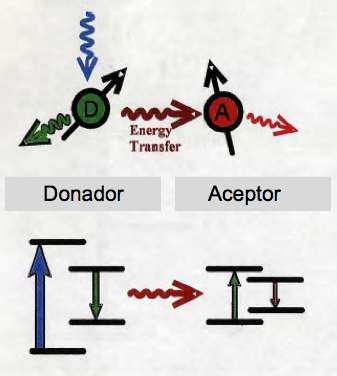
\includegraphics[width=0.5\textwidth]{capitulo2/fret}
\caption{\small{Esquema de la Transferencia de Energ\'ia de Resonancia F\"orster}\label{fretito}}   
\end{figure}

Los antecedentes de la t\'ecnica FRET comenzaron en 1922 con el trabajo experimental de Cario sobre lo que denomin\'o \emph{fluorescencia sensibilizada}. Cario introdujo vapor de mercurio y talio en un tubo de cuarzo, lo ilumin\'o utilizando una l\'ampara de mercurio a 253.5$nm$ y lo que observ\'o fue la emisi\'on de los \'atomos de talio;  en ausencia del mercurio, los \'atomos de talio no fueron excitados a dicha longitud de onda. %La transferencia de enrg\'ia fue explicada mediante colisiones de los \'atomos de ambos elementos.

Las primeras observaciones de fluorescencia sensibilizada en soluci\'on fueron realizadas por Jean Perrin y C. R. Choucroun en 1929. J. Perrin explic\'o la transferencia de energ\'ia por resonancia utilizando f\'isica cl\'asica y realiz\'o experimentos para analizar la polarizaci\'on de luz emitida por mol\'eculas en soluci\'on en funci\'on de la concentraci\'on. %A medida que la concentraci\'on aumentaba, la distancia promedio entre las mol\'eculas disminu\'ia, y por el aumento de probabilidad de transferencia de energ\'ia de excitaci\'on no radiativa, la polarizaci\'on medida se reduc\'ia.

En 1929 Kallmann y London presentaron una teor\'ia para explicar la transferencia de energ\'ia de resonancia desde el punto de vista de la mec\'anica cu\'antica. Esta teor\'ia consider\'o una interacci\'on de tipo dipolo--dipolo e introdujo el par\'ametro $R_0$ para referirse a la distancia entre el sistema donador y aceptor en la cual, la transferencia de energ\'ia y el decaimiento radiativo del sistema donador en estado excitado son igualmente probables. Kallmann y London calcularon que la probabilidad $P$ de que se presente una transferencia de energ\'ia es $P\propto \frac{1}{1+(\frac{R}{R_0})^6}$, donde $R$ es la distancia de separaci\'on que hay entre los dos sistemas en que se da la transferencia de energ\'ia. En 1932--1933 Francis Perrin expandi\'o la teor\'ia de Kallmann y London considerando las interacciones vibracionales de las mol\'eculas en soluci\'on, y fue en los a\~{n}os 40's cuando F\"orster public\'o una nueva versi\'on de la teor\'ia de transferencia de energ\'ia de resonancia con consideraciones semicl\'asicas y posteriormente con un tratamiento cu\'antico.

F\"orster concluy\'o, a diferencia de F. y J. Perrin, que no es posible asumir resonancia exacta entre dos \'atomos o mol\'eculas id\'enticas, ya que esto resultar\'ia en valores muy grandes de $R_0$ comparados con las mediciones experimentales; y realiz\'o correcciones utilizando la \emph{integral de traslape}, la cual se define como la superposici\'on del espectro de emisi\'on de la mol\'ecula donadora con el espectro de absorci\'on de la mol\'ecula aceptora (Ver Figura \ref{integral}). Con lo anterior se volvi\'o a definir la constante $R_0$ como la distancia F\"orster, siendo la separaci\'on molecular cr\'itica por debajo de la cual, hay transferencia de energ\'ia durante el tiempo de vida del estado excitado.

\begin{figure}[ht]
\centering
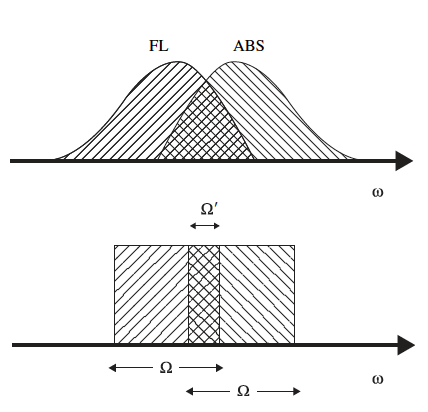
\includegraphics[width=0.6\textwidth]{capitulo2/overlap}
\caption{\small{Espectros de emisi\'on y absorci\'on de intensidad vs frecuencia, $\Omega'$ representa el ancho de la superposici\'on}\label{integral}}   
\end{figure}


La eficiencia de transferencia de energ\'ia de resonanacia F\"orster $E$ se define como la fracci\'on de fotones que son absorbidos por la mol\'ecula donadora y son transferidos a la mol\'ecula aceptora, o bien:

\begin{align}
E=\frac{1}{1+(R/R_0)^6}
\end{align}

F\"orster asumi\'o que el proceso de transferencia de energ\'ia no radiativa es mucho m\'as lento que la relajaci\'on vibracional entre los modos vibracionales del estado excitado debido a interacciones con el disolvente y determin\'o que la raz\'on de la transferencia de energ\'ia de resonancia $k_{D-A}$ puede expresarse como $k_{D-A}=\frac{1}{\tau_D} (\frac{R_0}{R})^6$, donde $\tau_D$ es el tiempo de vida medio de la mol\'ecula donadora en el estado excitado. 

La consideraci\'on de un acoplamiento d\'ebil entre dos osciladores: la mol\'ecula donadora y aceptora; o bien, de una interacci\'on d\'ebil de tipo dipolo--dipolo en la transferencia de energ\'ia de resonancia F\"orster, es lo que induce una transferencia de energ\'ia no radiativa e implica que las propiedades espectrales de la mol\'ecula donadora o aceptora no se vean afectadas \cite{megalibro}.

La t\'ecnica FRET se ha vuelto muy popular en estudios de biolog\'ia y qu\'imica, principalmente aplicada a microscop\'ia \'optica utilizando fluor\'oforos, ya que permite estudiar interacciones moleculares e interacciones entre pares de prote\'inas en c\'elulas vivas determinando las distancias que hay entre los sistemas donador y aceptor. En la mayor\'ia de aplicaciones la transferencia de energ\'ia de resonancia F\"orster se manifiesta en la disminuci\'on tanto del tiempo de vida como de la intensidad de fluorescencia del sistema donador acompa\~{n}ada de un incremento en la emisi\'on de fluorescencia del sistema aceptor.

%La transferencia de energ\'ia de resonancia F\"orster se puede presentar entre pares de \'atomos, mol\'eculas y agregados moleculares \cite{megalibro}.


\chapter{Desarrollo Experimental}   %\label{chap_content}
\minitoc

\section{Metodolog\'ia: Descripci\'on de caracterizaci\'on \'optica}


\begin{description}
\item[Fabricaci\'on de nanopart\'iculas.] Un grupo de materiales org\'anicos, que de acuerdo a su dise\~{n}o, podr\'ian presentar propiedades \'opticas de inter\'es para desarrollar marcadores biocompatibles, se utilizaron para fabricar suspensiones acuosas de nanopart\'iculas mediante el m\'etodo de reprecipitaci\'on. Se utilizaron principalmente semiconductores org\'anicos y mol\'eculas de tama\~{n}os variables.

\item[Caracterizaci\'on lineal.] Esta caracterizaci\'on \'optica de los materiales se realiz\'o en soluciones y en suspensiones acuosas de nanopart\'iculas; se adquirieron espectros de absorci\'on con un espectrofot\'ometro y espectros de emisi\'on lineal utilizando como excitaci\'on un diodo l\'aser de 370$nm$. Se midi\'o la eficiencia cu\'antica de fluorescencia utilizando el m\'etodo de la esfera integradora. 

\item[Caracterizaci\'on no lineal.] Se determin\'o la secci\'on transversal de absorci\'on de dos fotones $\sigma^{TPA}$ para soluciones y suspensiones de nanopart\'iculas del material precursor, utilizando la t\'ecnica de emisi\'on inducida por absorci\'on de dos fotones: se adquirieron espectros de emisi\'on no lineal utilizando l\'aseres de pulsos de femtosegundos en el rango espectral de inter\'es biom\'edico (730- 840$nm$ y/o 600- 900$nm$).

\item[Funcionalizaci\'on.] Las nanopart\'iculas que presentaron los valores m\'as\\ grandes de eficiencia cu\'antica de fluorescencia y de secci\'on transversal de absorci\'on de dos fotones se funcionalizaron utilizando polietilenglicol PEG. Este PEG (con m\'ultiples grupos funcionales) se utiliz\'o como agente surfactante y estabilizador y para recubrir y modificar la superficie de las nanopart\'iculas de los materiales precursores. 

\item[Fotoestabilidad.]  Se estudi\'o la fotoestabilidad degradando las nanopart\'iculas funcionalizadas en celdas de cuarzo de 1$mm$ con una l\'ampara de xen\'on de 150$W$ y monitoreando los espectros de absorci\'on a diferentes tiempos.

\item[Tinci\'on de c\'elulas con nanoparticulas.] Las suspensiones acuosas de\\ nanopart\'iculas funcionalizadas con PEG se internalizaron en l\'ineas celulares epiteliales y se obtuvieron im\'agenes de su distribuci\'on en la c\'elula con un microscopio de epifluorescencia. 

\end{description}

\section{Materiales y reactivos}\label{matis}

Se estudi\'o un grupo de 15 mol\'eculas fluorescentes sintetizados por la M.C. Mariana Flores y el Dr. Alejandro Alvarez Hern\'andez del Centro de Investigaciones en Qu\'imica, de la Universidad Aut\'onoma del Estado de Hidalgo; \'estas se basan en una mol\'ecula poliinsaturada con un grupo funcional amida y dos sustituyentes $R$. La estructura molecular y los 15 diferentes sustituyentes se muestran en la figura \ref{muchacha}.

Se trabaj\'o tambi\'en con un copol\'imero de dos bloques conocido como PF2/6-b-P3TMAHT, compuesto por el politiofeno
poli(9,9-dialquilfluoreno)-b-poli [3-(6-amoniohexil)tiofeno] (P3TMAHT) y el homopolifluoreno 2-(etil) hexil (PF2/6). Este copol\'imero, mostrado en la figura \ref{copolimerito}, fue proporcionado por el Dr. Ullrich Scherf de Bergische Universit\"at Wuppertal, Macromolecular Chemistry Group and Institute for Polymer Technology.

\begin{figure}[H]
\centering
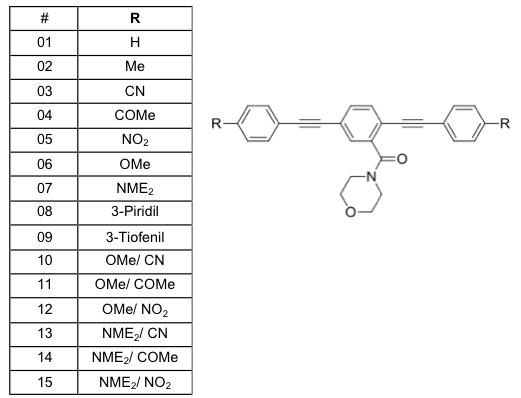
\includegraphics[width=0.85\textwidth]{desarrollo_experimental/HIDALGO}
\caption{15 sustituyentes $R$ en la estructura principal de la mol\'ecula \label{muchacha}}
\end{figure}


\begin{figure}[H]
\centering
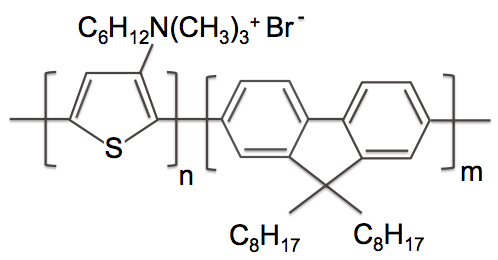
\includegraphics[width=0.55\textwidth]{desarrollo_experimental/copolimero}
\caption{Copol\'imero de dos bloques\label{copolimerito}}
\end{figure}



Por otra parte se estudiaron tres sistemas $\pi$ conjugados con diferente distribuci\'on de carga: etinilfluoreno-nitrilo (sistema dipolar) al que se har� referencia como 1NDS, etinilfluoreno-piridazina (sistema cuadrupolar) � 2NQS y etinilfluoreno-triazina (sistema octopolar) � 3NOS; en la figura \ref{ar2} se muestran las estructuras de estos sistemas basados en unidades de fluoreno. Los pesos moleculares $M_{w}$ son $515.771g/mol$, $905.387 g/mol$ y $1547.312g/mol$ para la mol\'ecula dipolar, cuadrupolar y octopolar respectivamente. Las mol\'eculas fueron dise\~{n}adas y sintetizadas por el Dr. Arturo Jim\'enez y la Dra. Rosa Santill\'an del Departamento de Qu\'imica Cinvestav- IPN.

\begin{figure}[h]
\centering
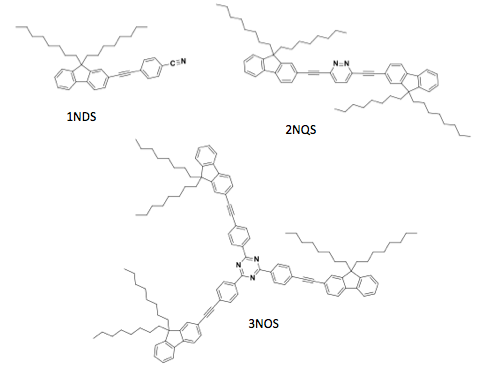
\includegraphics[width=\textwidth]{desarrollo_experimental/arturo}
\caption{Mol\'eculas org\'anicas dipolar, cuadrupolar y octopolar\label{ar2}}
\end{figure}

Finalmente se estudio tambi\'en el pol\'imero derivado de fluoreno PMC300 (Ver Figura \ref{PMC}), el cual est\'a basado en el mon\'omero 4,7-bis[2-(9,9-dimetil) fluorenil]benzo[1,2,5]tiadiazol; la s\'intesis se ha reportado por G. Ramos-Ort�z et al. \cite{laura}.

\begin{figure}[H]
\centering
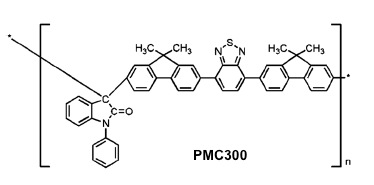
\includegraphics[width=0.7\textwidth]{desarrollo_experimental/PMC300}
\caption{Pol\'imero PMC300\label{PMC}}
\end{figure}

En este trabajo se utiliz\'o el colorante comercial Rodamina 6G de Sigma-Aldrich, principalmente como referencia (Ver estructura qu�mica en figura \ref{laroda}). La Rodamina 6G es una mol\'ecula fluorescente cuyas propiedades \'opticas lineales y no lineales han sido ampliamente estudiadas, tiene una eficiencia cu\'antica de fluorescencia de 0.95 y presenta una alta fotoestabilidad, adem\'as es un material que puede conseguirse f\'acilmente a un costo relativamente bajo.

\begin{figure}[H]
\centering
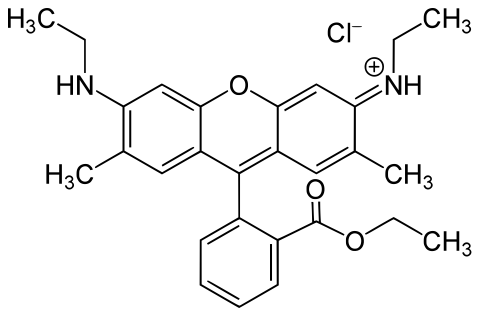
\includegraphics[width=0.55\textwidth]{desarrollo_experimental/rodamina6g}
\caption{Rodamina 6G\label{laroda}}
\end{figure}

Para recubrir las nanopart\'iculas se utilizaron dos tipos de polietilenglicol, PEG 5000 adquirido de Sigma-Aldrich y PEG 2000 de Avanti Polar Lipids Inc., el peso molecular promedio $M_n$ es de $5000g/mol$ y $2000g/mol$ respectivamente. Sus estructuras qu\'imicas se muestran en la figura \ref{pegs}.

\begin{figure}[H]
\centering
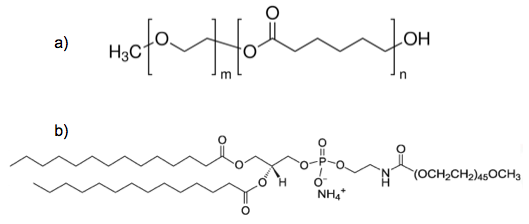
\includegraphics[width=0.85\textwidth]{desarrollo_experimental/peg}
\caption{Estructuras de a) PEG 5000 y b) PEG 2000 \label{pegs}}
\end{figure}


%poner que es thf, ctab y todos los nombres completos de los reactivos 

%peg 2000 y peg 5000


\section{Fabricaci\'on de nanopart\'iculas por el m\'etodo de reprecipitaci\'on}

El m\'etodo de reprecipitaci\'on se basa en la diferencia de solubilidad que tiene el material precursor en una mezcla compuesta por un buen disolvente y un mal disolvente para dicho precursor, ambos miscibles \cite{reprecipita}. La creaci\'on de este sistema mediante una mezcla r\'apida provoca una precipitaci\'on local y la nucleaci\'on de nanopart\'iculas en lugar de una precipitaci\'on en bulto \cite{coloidal}.

El proceso de reprecipitaci\'on para la fabricaci\'on de suspensiones acuosas de nanopart\'iculas de los sistemas org\'anicos a estudiar (Ver Figura \ref{fig_repreci}), es el siguiente:

\begin{description}
\item[$\circ$]  Preparaci\'on de una soluci\'on madre en THF a una concentraci\'on de $1\times10^{-3}$ \'o $1\times10^{-4} M$ dependiendo del peso molecular del material precursor.
\item[$\circ$]  Se realiz\'o una soluci\'on de un surfactante en agua a una concentraci\'on de 0.8 $mM$. El surfactante m\'as utilizado fue el CTAB aunque tambi\'en se realizaron pruebas con Trit\'on- X 100  
\item[$\circ$]  Utilizando jeringas de insulina se inyectaron r\'apidamente 0.5$ml$ de la soluci\'on madre en 8$ml$ de la soluci\'on acuosa bajo sonicaci\'on para causar la nucleaci\'on de nanopart\'iculas a una concentraci\'on de $1\times10^{-5}$ a $1\times10^{-7} M$ dependiendo del material.
\item[$\circ$]  Como se busc\'o desarrollar marcadores biocompatibles, se evapor\'o el disolvente t\'oxico de la suspensi\'on acuosa de nanopart\'iculas\footnote{De acuerdo con la literatura, �ste tipo de m�todo de fabricaci�n de nanopart�culas puede desarrollar marcadores o portadores de f�rmacos biocompatibles al evaporar el disolvente, ya que el surfactante recubre las nanopart�culas del material precursor y cambia la solubilidad de �ste �ltimo, en agua. Ver por ejemplo referencia \cite{artconcluyente}.}. La suspensi\'on se introdujo en un matraz de Kitasato haciendo vac\'io con una bomba de extracci\'on.
\end{description}

\begin{figure}[H]
\centering
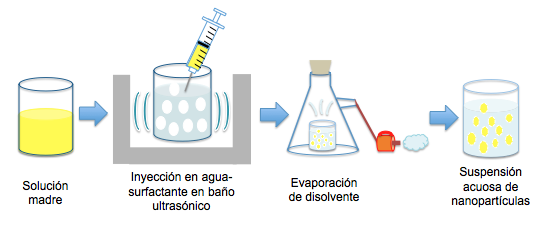
\includegraphics[width=1\textwidth]{desarrollo_experimental/reprecipitacion}
\caption{M\'etodo de reprecipitaci\'on}\label{fig_repreci}
\end{figure}

El surfactante act\'ua como un agente estabilizador en la suspensi\'on acuosa de nanopart\'iculas. El tama\~{n}o de \'estas se puede controlar  modificando la concentraci\'on de la soluci\'on madre y el disolvente.

\subsection{Recubrimiento de nanopart\'iculas con PEG}\label{pegis}

Los dos tipos de PEG que se utilizaron en este trabajo son anfif�licos y tienen los grupos funcionales: \'eter, \'ester y alcohol en el caso del PEG 5000 y \'ester, varios grupos \'eter, fosfato, amonio y amida en el PEG 2000 (Grupos funcionales mencionados de izquierda a derecha en las estructuras de la figura \ref{pegs}). As�, al utilizarlos para recubrir las nanopart\'iculas, se modific� la superficie de las mismas y se llev� a cabo una funcionalizaci\'on.

Para realizar la funcionalizaci�n de nanopart�culas se utiliz� el m�todo de reprecipitaci�n (Ver Figura \ref{fig_repreci}), reemplazando al surfactante por PEG. Con el PEG 5000 se prepar\'o una soluci\'on acuosa a una concentraci\'on de $4\times10^{-6} M$, debido a que \'este se precipitaba en soluciones acuosas a concentraciones mayores o iguales a $1\times10^{-5} M$. Y nuevamente a 8$ml$ de \'esta soluci\'on se inyectaron 0.5$ml$ de la soluci\'on madre del material precursor de inter\'es, para formar una suspensi\'on acuosa de nanopart\'iculas funcionalizadas con este PEG a concentraciones del orden de $10^{-6} M$. Posteriormente el disolvente fue evaporado.

El PEG 2000 present\'o m\'as estabilidad, para este caso la soluci\'on acuosa pudo prepararse a una concentraci\'on de $6\times10^{-4} M$ (Concentraci\'on del orden de magnitud m\'as reportado en la literatura). Las suspensiones acuosas de nanopart\'iculas tuvieron concentraciones entre $10^{-6}$ y $10^{-7} M$, inyectando 0.5$ml$ de la soluci\'on madre en 8 $ml$ de la soluci\'on acuosa y despu\'es de evaporar el disolvente.

%\subsubsection{Transferencia de energ\'ia de resonancia F\"orster}

%\subsubsection{PEG 5000}
%Con este PEG se funcionalizaron las nanopart\'iculas de la mol\'ecula octopolar 3NOS. Inicialmente se prepar\'o la soluci\'on madre a una concentraci\'on de $1\times10^{-4} M$ y se realiz\'o una soluci\'on acuosa de PEG 5000 a una conc�ntrica\'on de $4\times10^{-6} M$. Se inyectaron 0.5$ml$ de soluci\'on madre en 8$ml$ de la soluci\'on acuosa para obtener una suspensi\'on acuosa de nanopart\'iculas a una concentraci\'on de $6.4\times10^{-6} M$ y posteriormente se evapor\'o el disolvente.

%\subsubsection{PEG 2000}
%Las nanopart\'iculas del pol\'imero PMC300, PMC300 dopado con Rodamina 6G, de la mol\'ecula octopolar y del dendr\'imero se funcionalizaron con PEG 2000. Se prepararon las soluciones madre del pol\'imero PMC300 a una concentraci\'on de $5.9\times10^{-6} M$; una soluci\'on de este pol\'imero (misma concentraci\'on) dopada con Rodamina 6G al 177, 100 y 50\% molar; la soluci\'on de la mol\'ecula octopolar a $1\times10^{-4} M$  y del dendr\'imero a una concentraci\'on de $1.1\times10^{-4} M$.

%En este caso, la soluci\'on acuosa de PEG 2000 se prepar\'o a una concentraci\'on de $1\times10^{-4} M$. 

%Se inyectaron 0.5$ml$ de las soluciones madre en 8$ml$ de las soluciones acuosas para cada compuesto; obteniendo  suspensiones acuosas con concentraciones de $3.5\times10^{-7} M$,$3.5\times10^{-7} M$ de PMC300/ $1.75\times10^{-7} M$ de Rodamina 6G, de $6.4\times10^{-6} M$ y de $6.9\times10^{-6} M$ para las nanopart\'iculas de PMC300, PMC300 con Rodamina 6G al 50\% molar, de la mol\'ecula octopolar y el dendr\'imero respectivamente. Posteriormente se evapor\'o el disolvente.
\section{Espectros de absorci\'on y emisi\'on lineal}

Los espectros de absorci\'on de las soluciones y suspensiones acuosas de nanopart\'iculas se obtuvieron con el espectrofot\'ometro  Perkin Elmer modelo Lambda 900 en un rango de 250 a 900 $nm$. Las soluciones y suspensiones se colocaron en celdas de cuarzo de $0.1\times1\times4 cm^{3}$ \'o $1\times1\times4 cm^{3}$ dependiendo de la concentraci\'on y la absorbancia de cada muestra.

Los espectros de emisi\'on lineal se obtuvieron con un espectr\'ometro port\'atil Ocean Optics USB4000, excitando las muestras con un diodo l\'aser emitiendo a 370$nm$ como se muestra en la figura \ref{emilineal}. El haz de excitaci\'on enfocado con la lente L1 incide en la muestra contenida en la celda, la luz emitida es recolectada con un sistema de lentes perpendicular al haz de excitaci\'on; la lente L2 colecta la fluorescencia y la colima; la lente L3 forma la imagen del volumen excitado en la abertura del espectrometro. El espectrometro est\'a sobre una montura XY que permite su alineaci\'on para detectar mayor fluorescencia y utilizando el programa Spectra Suite, se pueden visualizar y guardar los espectros de emisi\'on.

\begin{figure}[h]
\centering
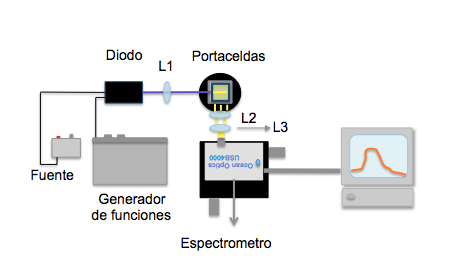
\includegraphics[width=0.9\textwidth]{desarrollo_experimental/emision_lineal}
\caption{Arreglo experimental para medir emisi\'on lineal}\label{emilineal}
\end{figure}

Es necesario guardar un espectro de emisi\'on con el diodo l\'aser apagado para detectar la se\~{n}al de fondo y restarla de los espectros de emisi\'on obtenidos para cada muestra. 

El diodo l\'aser se modul\'o con un generador de funciones: amplitud de 0 $Vpp$ y un Offset de 1V. Para evitar la saturaci\'on del espectrometro se utilizaron filtros neutros de densidad \'optica variable entre la fuente de excitaci\'on y la muestra o bien, se redujo el valor del offset. 

\section{Medici\'on de eficiencia cu\'antica de fluorescencia}

La eficiencia cu\'antica de fluorescencia de los materiales estudiados se midi\'o en soluciones y/o suspensiones de nanopart\'iculas, colocando \'estas en una celda de cuarzo de $0.1\times1\times4 cm^{3}$. En el arreglo experimental se utiliz\'o un diodo l\'aser a 370$nm$ como fuente de excitaci\'on, un diafragma $D1$, dos lentes $L1$ y $L2$, una esfera integradora de 25.4$cm$ de di\'ametro interno, modelo INS250 de International Light Technologies; un tubo fotomultiplicador o PMT por sus siglas en ingles (serie R7400U de Hamamatsu) colocado a 90$^{\circ}$ del haz de excitaci\'on y un amplificador lock- in modelo SR830 de Stanford Research Systems, como se muestra en la figura \ref{eficiencia}. 

\begin{figure}[h]
\centering
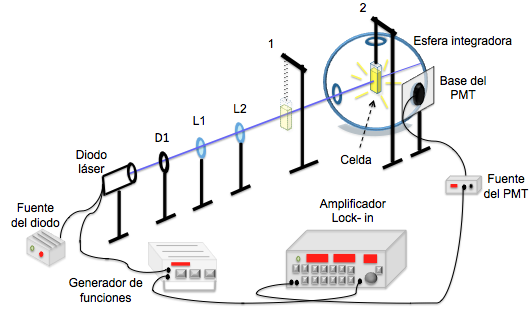
\includegraphics[width=1\textwidth]{desarrollo_experimental/arreglo_qy}
\caption{Arreglo experimental para obtener la eficiencia cu\'antica de fluorescencia}\label{eficiencia}
\end{figure}

El diodo l\'aser de 370$nm$ se modul\'o con el generador de funciones utilizando regularmente una se\~{n}al cuadrada con frecuencia de 60$Hz$, amplitud de 1$Vpp$ y offset de 0.5$V$; \'esta se\~{n}al se utiliz\'o como referencia en el amplificador lock- in. Con el diafragma $D1$ se realiz\'o un filtrado espacial de la luz, la lente $L1$ enfoc\'o el haz y la lente $L2$ se utiliz\'o para colimar la luz. La celda se coloc\'o en bases fijas fuera y dentro de la esfera (Ver Figura \ref{eficiencia}) en las posiciones 1 y 2 respectivamente. 

En la esfera, a pesar de los filtros, la luz reflejada internamente proviene del haz de excitaci\'on residual, fluorescencia de la muestra y ruido; y es detectada por el PMT\footnote{El PMT se encendi\'o utilizando 200 V en todas las mediciones}. Sin embargo, en el amplificador lock- in se utiliz\'o la frecuencia del generador de funciones como referencia para discriminar el ruido y luz proveniente de otras fuentes. Los valores entregados por el lock- in se dieron en volts $V$.

Se utiliz\'o Rodamina 6G (Ver Figura \ref{laroda}) como colorante de referencia para calcular las eficiencias cu\'anticas de los compuestos de inter\'es. La celda se coloc\'o en las posiciones 1 y 2 mostradas en la figura \ref{eficiencia} para detectar solamente la fluorescencia: en la posici\'on 2, la luz de excitaci\'on transmitida por la celda, fluorescencia del compuesto y ruido se detectaron; mientras que en la posici\'on 1 solo la luz de excitaci\'on transmitida y el ruido. Entonces para cada muestra (incluida la referencia) se rest\'o el valor arrojado por el amplificador en la posici\'on 1 al valor obtenido en la posici\'on 2 y obtener idealmente  luz emitida por el compuesto en soluci\'on o suspensi\'on.

La superficie de mayor \'area en la celda se aline\'o perpendicular a la direcci\'on de propagaci\'on de la luz de excitaci\'on para evitar que el haz reflejado se quedara en el interior de la esfera integradora.
 
Debido a la sensibilidad del PMT, este s\'olo se encend\'ia hasta que la celda era colocada en las posiciones preestablecidas y despu\'es de ser alineadas con el haz de excitaci\'on. Para evitar da\~{n}ar este fotomultiplicador solo se dejaba encendido el instante en el que se registraban los valores arrojados por el amplificador. Se intentaba aislar de cualquier tipo de luz externa el sitio en el que se mont\'o el arreglo experimental mientras el PMT se encontraba encendido. Adem\'as la pantalla dentro de la esfera, entre la muestra y el sistema de detecci\'on, se utiliz\'o para proteger el PMT de la detecci\'on directa de la luz de excitaci\'on y/o fluorescencia; tambi\'en se colocaron filtros UV entre la salida de la esfera y el PMT, para atenuar la luz de excitaci\'on.

Las soluciones y suspensiones acuosas de nanopart\'iculas con las que se trabaj\'o, ten\'ian concentraciones bajas de $1\times10^{-5}$ a $1\times10^{-7} M$ para evitar interacciones y procesos, que por la proximidad de las  mol\'eculas, pudieran  llevar a la disminuci\'on de fluorescencia. En las muestras que aun a bajas concentraciones presentaban una gran emisi\'on de luz se utilizaron filtros neutros de densidad \'optica variable o se modificaban los par\'ametros del generador de funciones (para as\'i disminuir el nivel de excitaci\'on).

\section{Medici\'on de \texorpdfstring{$\sigma^{TPA}$}{sigmaTPA} de 740 a 840 nm}\label{laserlau}

La secci\'on transversal de absorci\'on de dos fotones de las suspensiones acuosas de nanopart\'iculas y soluciones del material de inter\'es se midieron mediante la t\'ecnica de TPEF, adquiriendo los espectros de emisi\'on inducida por absorci\'on de dos fotones. Para ello se utiliz\'o un l\'aser de Titanio: Zafiro con pulsos de 100 $fs$ de duraci\'on y frecuencia de repetici\'on de 80 $MHz$ en un rango de 725-- 860 $nm$ (modelo \emph{Tsunami}-3955 de Spectra-Physics); este l\'aser fue bombeado por un l\'aser de onda continua \emph{Millennia Pro s- Series} a 532 $nm$ con una potencia de 5 Watts.

En la figura \ref{sencillotpa} se aprecia el arreglo experimental; a la salida del l\'aser de Ti:Za se coloc\'o un retardador de media longitud de onda y un aislador de Faraday (componente $A$) para controlar la intensidad de excitaci\'on, se desvi\'o el haz utilizando cuatro espejos $M1$-$M4$ para no interferir con otros arreglos colocados sobre la mesa \'optica de trabajo, el diafragma $D1$ se utiliz\'o como referencia para alinear los componentes \'opticos, la lente $L1$ enfoc\'o el haz en una celda de cuarzo de $1\times1\times4 cm^3$ con la soluci\'on o suspensi\'on de inter\'es y con el sistema de lentes $L2$ y $L3$, colocadas de manera perpendicular al haz incidente, se colect\'o y dirigi\'o la fluorescencia inducida por absorci\'on de dos fotones a la abertura del espectr\'ometro port\'atil Ocean Optics USB4000. 

Idealmente la lente $L2$ colima la luz mientras que la lente $L3$ la enfoca en la abertura del espectrometro, \'este se encontraba sobre una montura XY para detectar la mayor cantidad de fluorescencia, y para visualizar y guardar los espectros de emisi\'on se utiiz\'o el programa Spectra Suite. El haz de excitaci\'on se enfoc\'o en un extremo de la celda de cuarzo, muy cercano a una de sus paredes para reducir la distancia entre el volumen excitado y las lentes colectoras de luz, disminuyendo as\'i la atenuaci\'on de fluorescencia debida a efectos de absorci\'on.

\begin{figure}[h]
\centering
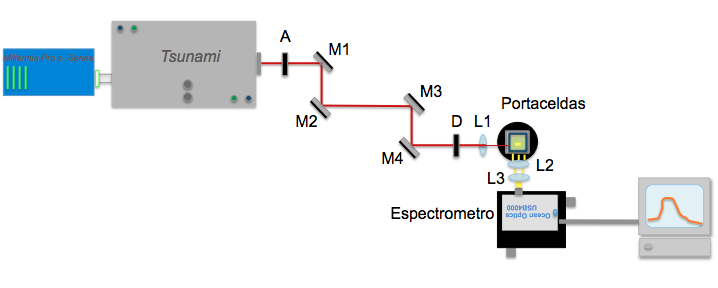
\includegraphics[width=1\textwidth]{desarrollo_experimental/tpa}
\caption{Arreglo experimental para medir $\sigma^{TPA}$ (Rango 740-- 840 $nm$)}\label{sencillotpa}
\end{figure}

Como muestra de referencia se utiliz\'o  Rodamina 6G a una concentraci\'on de $1\times 10^{-4} M$. Los espectros de emisi\'on no lineal de las nanopart\'iculas o soluciones y de la referencia, fueron obtenidos bajo las mismas condiciones con una potencia incidente de 410 $mW$ \footnote{Esta potencia se midi\'o a la salida del aislador de Faraday} y para 11 diferentes longitudes de onda de excitaci\'on: de 740 a 840 $nm$ cada 10 $nm$. Adem\'as, para cada longitud de onda se guard\'o la se\~{n}al detectada por el espectrometro al bloquear el haz de excitaci\'on para restar esta se\~{n}al de fondo a los espectros de cada muestra incluida la referencia. 

El l\'aser de Ti:Za se sintoniz\'o girando dos tornillos de movimiento microm\'etrico ubicados en la parte superior del l\'aser. Uno de ellos cambia la posici\'on de una rendija que modifica la longitud de onda y el otro tornillo mueve un compensador de dispersi\'on, formado por cuatro prismas.

\section{Medici\'on de \texorpdfstring{$\sigma^{TPA}$}{sigmaTPA} de 650 a 760 nm}\label{laserchidote}

Para medir $\sigma^{TPA}$ en este rango mediante la t\'ecnica TPEF se utiliz\'o un amplificador ultrarr\'apido (basado en un l\'aser de Ti:Za) modelo Libra- HE de Coherent, con emisi\'on de pulsos de 50 $fs$ de duraci\'on, frecuencia de repetici\'on de 1 $kHz$ y longitud de onda central de 800nm; adicionalmente se utiliz\'o un amplificador \'optico param\'etrico modelo TOPAS- C de Light Conversion capaz de sintonizar la longitud de onda en un rango continuo de 290 a 2600 $nm$. Como sistema de detecci\'on se utiliz\'o un monocromador/espectr\'ometro de la serie Acton SP-2500i de Princeton Instruments y un tubo fotomultiplicador o PMT por sus siglas en ingles de la serie R7400U de Hamamatsu.


Como se aprecia en la figura \ref{mastpa} el amplificador \'optico param\'etrico TOPAS- C fue bombeado por el l\'aser Libra- HE utilizando los espejos $M1$-$M4$, el TOPAS- C se sintoniza y controla utilizando un programa computacional del equipo y a la salida de \'este, se coloca el filtro correspondiente para permitir la salida de la longitud de onda seleccionada. Utilizando el espejo $M5$, el haz de excitaci\'on se envi\'o a una serie de filtros de densidad \'optica variable para controlar la intensidad del haz y posteriormente el haz se modul\'o utilizando un chopper $C$ a una frecuencia de 39 $Hz$. Con los espejos $M6$ y $M7$ el haz se hizo incidir en la lente $L1$ para ser enfocado en una celda de cuarzo de $1\times1\times4 cm^3$; con las lentes $L2$- $L3$ se colect\'o la luz emitida por la muestra de inter\'es de manera perpendicular al haz incidente en la celda; utilizando los espejos $M8$-$M10$ la luz emitida se dirigi\'o a la lente $L4$ para enfocarla en la rendija de entrada del monocromador/ espectr\'ometro $M$ utilizando el espejo $M11$. 

\begin{figure}[h]
\centering
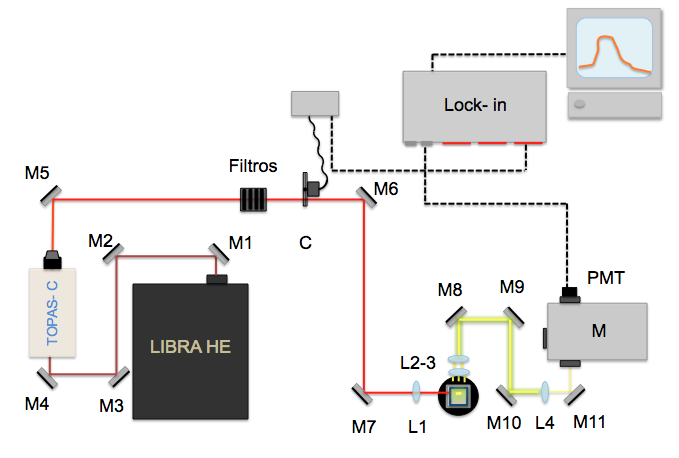
\includegraphics[width=1\textwidth]{desarrollo_experimental/tpa_femto}
\caption{Arreglo experimental para medir $\sigma^{TPA}$ (Rango 650-- 760 $nm$)}\label{mastpa}
\end{figure}



A la salida del monocromador/ espectr\'ometro se coloc\'o un PMT, encendido con 900 $V$ en todas las mediciones, y se amplific\'o la se\~{n}al detectada con un amplifciador lock- in modelo SR830 de Stanford Research Systems, utilizando como referencia la se\~{n}al del chopper. Para poder visualizar y guardar los espectros de emisi\'on en base a los datos del amplificador lock- in, se utiliz\'o un software desarrollado por un miembro del GPOM\footnote{El software fue desarrollado por el Ing. f\'isico Manuel De Anda Villa para automatizar la detecci\'on y guardado de datos arrojados por el Lock-in de forma gr\'afica}. El haz de excitaci\'on se enfoc\'o muy cerca a una de las paredes de la celda de cuarzo para reducir la distancia entre el volumen excitado y las lentes colectoras de luz, disminuyendo as\'i la atenuaci\'on de fluorescencia.

Se utiiz\'o nuevamente Rodamina 6G como referencia a una concentraci\'on de $1\times 10^{-4} M$. Los espectros de emisi\'on no lineal de la muestra de referencia, suspensiones acuosas de nanopart\'iculas y soluciones fueron obtenidos bajo las mismas condiciones con una potencia incidente de entre 250 y 270 $\mu W$ para 12 diferentes longitudes de onda de excitaci\'on: de 650 a 760 $nm$ cada 10 $nm$. Y nuevamente para cada longitud de onda se guard\'o un espectro de la se\~{n}al detectada al bloquear el haz de excitaci\'on, para restar \'este fondo a los espectros de cada muestra de inter\'es incluida la referencia.

La medici\'on de $\sigma^{TPA}$ en este rango no se realiz\'o para todos los materiales estudiados, \'unicamente para los materiales de mayor inter\'es que presentaron los valores m\'as altos de $\sigma^{TPA}$ para el rango de 740 a 840 $nm$.

\section{Fotoestabilidad de las nanopart\'iculas}\label{fotitopalalupe}

Las soluciones y suspensiones acuosas de nanopart\'iculas de mayor inter\'es fueron sometidas a un estudio de fotoestabilidad; las muestras fueron expuestas a una l\'ampara UV durante 165 minutos, monitoreando los espectros de absorci\'on a diferentes tiempos. Las muestras se colocaron a 15 $cm$ de la l\'ampara para evitar que se calentaran demasiado y el disolvente se evaporara. 

El objetivo de este estudio fue comprobar que las soluciones sufren de un fotoblanqueado en un tiempo menor de exposici\'on a la luz comparadas con las suspensiones acuosas de nanopart\'iculas del mismo material.

\section[Internalizaci\'on de nanopart\'iculas en l\'ineas celulares epiteliales]{Internalizaci\'on de nanopart\'iculas en l\'ineas celulares epiteliales (L929)}\label{yacasicasi}

Las c\'elulas epiteliales L929 (Fibroblastos de rat\'on) son cultivadas\footnote{Se cont\'o con el apoyo de la Dra. Myrna Sabanero L\'opez del Laboratorio de Biolog\'ia Celular y Molecular de las Interacciones, de la Universidad de Guanjauato; la Dra. Sabanero proporcion\'o las l\'ineas celulares y desarroll\'o el protocolo y proceso de la tinci\'on celular.} en un medio DMEM (Dulbecco's Modified Eagle's Medium), el cual contiene amino\'acidos, sal, vitaminas, glucosa, hierro y rojo de fenol, suplementado con 10\% de suero fetal bovino y 0.1\% de antibi\'oticos y antimic\'oticos. Los cultivos se incubaron a una temperatura de 37$^{\circ} C$, con una atm\'osfera de 5\% de CO$_2$ y humedad constante.

Las nanopart\'iculas org\'anicas de mayor inter\'es por sus propiedades \'opticas, se internalizaron en las lineas celulares siguiendo el protocolo siguiente:

\begin{description}
\item[1.-]  Las c\'elulas se fijaron en cubreobjetos de 20$\times$20 $mm$ utilizando paraformaldehido 4\% y glutaraldehido 0.05\% en una soluci\'on salina de fosfato (PBS) durante 20 minutos.
\item[2.-]  Las c\'elulas fueron permeabilizadas utilizando Trit\'on 0.05\% durante tres minutos.
\item[3.-]  Se prepar\'o una sonda compuesta por suero fetal bovino y suspensi\'on acuosa de nanopart\'iculas en diferentes proporciones.
\item[4.-]  Las c\'elulas fueron expuestas a la sonda por un tiempo de 30 minutos.
\item[5.-]  El cubreobjetos con las c\'elulas y la sonda fue montado y sellado en un portaobjetos, adicionando DAPI (4 ',6-diamino-2-fenilindol) entre las laminillas. El DAPI es un marcador fluorescente que se une fuertemente al ADN o bien al n\'ucleo de las c\'elulas.
\item[6.-]  Finalmente el portaobjetos, con las nanopart\'iculas en las c\'elulas, se observ\'o con el microscopio de epifluorescencia modelo IX81 de Olympus.
\end{description}

Cabe mencionar que posterior al paso n\'umero 1, 2 y 4 las c\'elulas del cubreobjetos fueron lavadas suavemente utilizando PBS, ello para remover las c�lulas que no se fijaron, para retirar el surfactante no absorbido y limpiar las c�lulas de las nanopart�culas que no se internalizaron.




%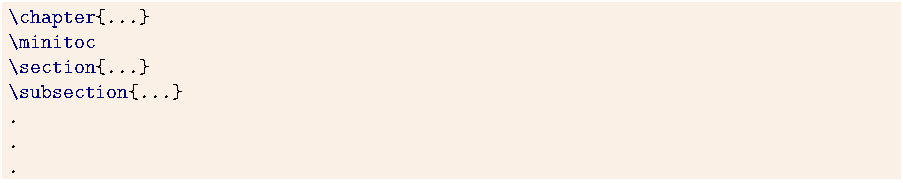
\includegraphics[width=\textwidth]{your_stuff/pre}


\chapter{Resultados}   
\minitoc

\section{Propiedades \'opticas de algunas mol\'eculas $\pi$ conjugadas}

En la figura \ref{muchacha} se muestra una estructura de bajo peso molecular con un grupo de 15 sustituyentes distintos $R$ en dos de sus extremos; este conjunto de mol\'eculas fue estudiado en soluci\'on y suspensi\'on. La concentraci\'on de las soluciones y suspensiones acuosas fue del orden de $10^{-5} M$ y en la fabricaci\'on de las mismas se utiliz\'o Trit\'on X- 100 como surfactante, debido a que se observaron mejores resultados que utilizando CTAB (Suspensiones m\'as transparentes y estables).

No todas las mol\'eculas fueron solubles en THF, tampoco se pudieron fabricar suspensiones acuosas de nanopart\'iculas en todos los casos porque se formaban grandes aglomerados que se precipitaban y en algunos casos la emisi\'on lineal fue d\'ebil. En la figura \ref{abshgo} se muestran los espectros de absorci\'on lineal molar $\epsilon$ de las soluciones y suspensiones m\'as estables que presentaron mayor emisi\'on, en \'estos se puede observar el esparcimiento de las suspensiones. La absorci\'on disminuy\'o notoriamente en la mol\'ecula 7 en suspensi\'on comparada con la soluci\'on, mientras que para la mol\'ecula 3 el espectro de absorci\'on  de la suspensi\'on present\'o mayor intensidad de emisi\'on, un corrimiento hacia el rojo y ensanchamiento (debido a la torsi\'on y/o flexi\'on que sufre la mol\'ecula) en comparaci\'on con la soluci\'on.

\begin{figure}[h]
\centering
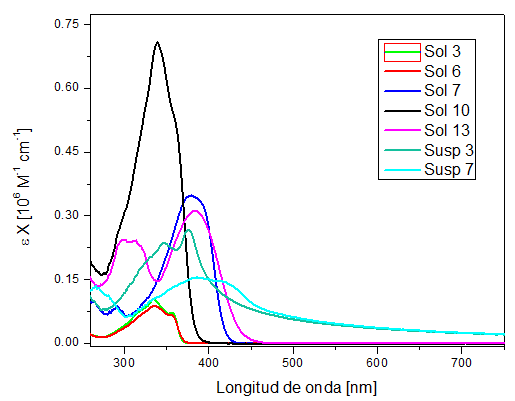
\includegraphics[width=0.9\textwidth]{resultados/sechgo/abstodas}
\caption{Espectros de absorci\'on molar de las mol\'eculas 3, 6, 7, 10, 13 y 15 (Notaci\'on de acuerdo a la fig. \ref{muchacha}). Las etiquetas \emph{Sol} y \emph{Susp} se refieren a las mol\'eculas en soluci\'on y suspensi\'on respectivamente.}\label{abshgo}
\end{figure}

En la figura \ref{emilinhgo} se muestran los espectros de emisi\'on lineal. El espectro de la soluci\'on 6 present\'o una intensidad mayor que la soluciones 10 y 13, sin embargo, se traslap\'o con la emisi\'on del diodo l\'aser de 370 $nm$ y como se utiliz\'o un filtro UV para no detectar la fuente de excitaci\'on, el espectro de la soluci\'on 6 no se pudo visualizar por completo. Lo mismo sucedi\'o para el espectro de la mol\'ecula 3 en soluci\'on, mientras que en suspensi\'on tuvo un corrimiento hacia el rojo por las interacciones que sufre la mol\'ecula al confinarse para formar las nanopart\'iculas. El espectro de la mol\'ecula 7 en suspensi\'on tambi\'en sufri\'o un corrimiento hacia el rojo comparado con el espectro en soluci\'on.

Como las mol\'eculas 3, 6, 7, 10 y 13 en soluci\'on presentaron la mayor intensidad de emisi\'on lineal, pudiendo disolverse f\'acilmente en THF y las mol\'eculas 3 y 7 formaron las suspensiones acuosas m\'as transparentes y estables (Ver Figura \ref{susphgo}), \'unicamente se midi\'o la eficiencia cu\'antica de fluorescencia para estas mol\'eculas; los resultados se muestran en la tabla \ref{tablahgo}.




\begin{figure}[H]
\centering
\begin{subfigure}{\textwidth}
\centering
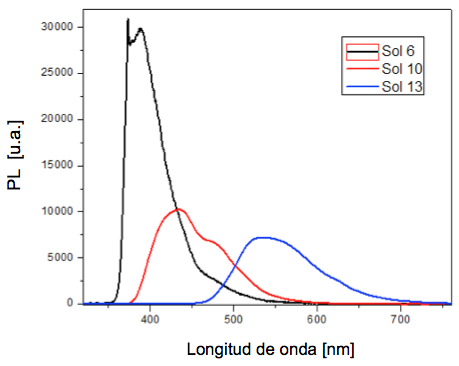
\includegraphics[width=0.65\textwidth]{resultados/sechgo/emlinsol}
\end{subfigure}
\begin{subfigure}{\textwidth}
\centering
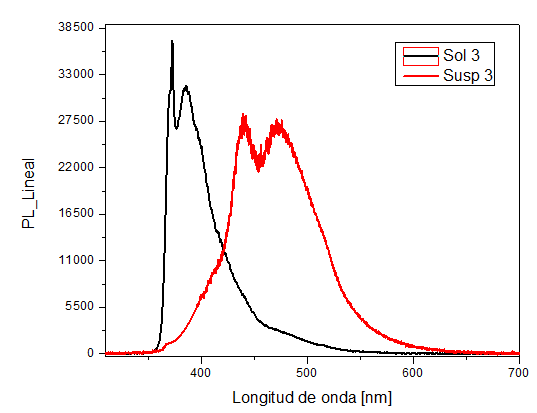
\includegraphics[width=0.65\textwidth]{resultados/sechgo/m3}
\end{subfigure}
\begin{subfigure}{\textwidth}
\centering
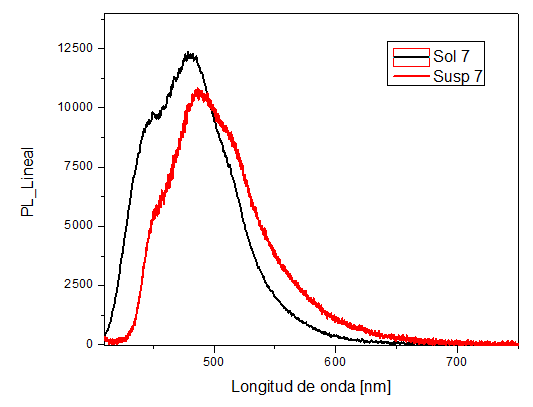
\includegraphics[width=0.65\textwidth]{resultados/sechgo/m7}
\end{subfigure}
\caption{Espectros de emisi\'on lineal de las muestras 6, 10 y 13 en soluci\'on y de las muestras 3 y 7 en soluci\'on y suspensi\'on de nanopart\'iculas.}
\label{emilinhgo}
\end{figure}

\begin{figure}[h]
\centering
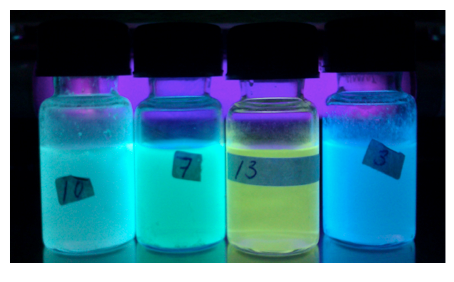
\includegraphics[width=0.45\textwidth]{resultados/sechgo/suspturbias}
\caption{De izquierda a derecha, fluorescencia de las muestras 10, 7, 13 y 3 en suspensi\'on bajo una l\'ampara UV como fuente de excitaci\'on.}\label{susphgo}
\end{figure}


La \'ultima columna de la tabla \ref{tablahgo} hace referencia al valor de $\Phi_f$ promedio tomando en cuenta un factor de correcci\'on\footnote{Este factor de correcci\'on se obtiene de las curvas de respuesta del PMT contenidas el manual de dicho equipo} proveniente de la sensibilidad de respuesta que el PMT tiene para distintas longitudes de onda. Es decir,  cuando la fluorescencia de la muestra de inter\'es y de la referencia (Rodamina 6G) tienen longitudes de onda similares, el PMT responder\'a de la misma manera en ambas muestras; sin embargo, si la muestra y la referencia emiten a diferentes longitudes de onda, es necesario introducir un factor de correci\'on.



\begin{table}[h]
\centering
\scalebox{0.82}{
\begin{tabular}{| l | c | c | c | c | c | r | }  %p{6.5cm} | c |
\hline
Muestra          & $\Phi_{f1}$ &$\Phi_{f2}$& $\Phi_{f Promedio}$&$\Phi_{fPromedio}$ /correcci\'on PMT  \\ \hline   %\multicolumn{8}{|c|}
Sol 3 	& 0.154	& 0.141	&0.148 & 0.09 \\ \hline
Sol 6         & 0.120     & 0.105	& 0.113 & 0.07    \\ \hline
Sol 7         & 0.430     & 0.236	& 0.333 & 0.20    \\ \hline
Sol 10 	& 0.266	& 0.255	&0.260 & 0.16 \\ \hline
Sol 13 	& 0.237	& 0.297	&0.267 & 0.27   \\ \hline
Susp 3 	& 0.279	& 0.148	&0.213 & 0.13    \\ \hline
Susp 7      &0.357     & 0.311      &0.335& 0.22  \\ \hline
\end{tabular} } 
\caption{ Valores obtenidos de eficiencia cu\'antica de fluorescencia $\Phi_f$ de las soluciones 3, 6, 7, 10 y 13 y las suspensiones 3 y 7.\label{tablahgo}}
\end{table}

Posteriormente se realizaron mediciones de $\sigma^{TPA}$ en un rango de 750 a 810 $nm$, para determinar \'este par\'ametro mediante la t\'ecnica de TPEF se utiliz\'o la ecuaci\'on \ref{finalsigma}, sin embargo, como los espectros de emisi\'on no lineal de la muestra de inter\'es y de referencia se adquirieron bajo las mismas condiciones, utilizando el mismo sistema de detecci\'on, entonces $\eta_{ref}=\eta$; de igual manera, la potencia incidente fue la misma para todas las muestras $\langle P(t)\rangle_{ref}=\langle P(t)\rangle$. Los valores de $\sigma^{TPA}_{ref}$ para la Rodamina 6G, a diferentes longitudes de onda, ya se encuentran reportados en la literatura (Ver referencia \cite{rusitos}). Si se asume que $n_{ref}/n\approx 1$, el par\'ametro a calcular para conocer $\sigma^{TPA}$ es el valor de la integral del espectro de emisi\'on no lineal de la referencia y de la muestra de inter\'es $\langle F(t)\rangle_{ref}$ y $\langle F(t)\rangle$.

Las soluciones 3, 6, 13 y la suspensi\'on 3 no presentaron fluorescencia inducida por absorci\'on de dos fotones en el rango mencionado con anterioridad; sin embargo, los espectros de emisi\'on no lineal de las soluciones 7, 10, 13 y la suspensi\'on 7 se detectaron a todas las longitudes de onda de excitaci\'on. En la figura \ref{eminlhgo} se muestran los espectros adquiridos con una longitud de onda de excitaci\'on de 750 $nm$. 

\begin{figure}[h]
\centering
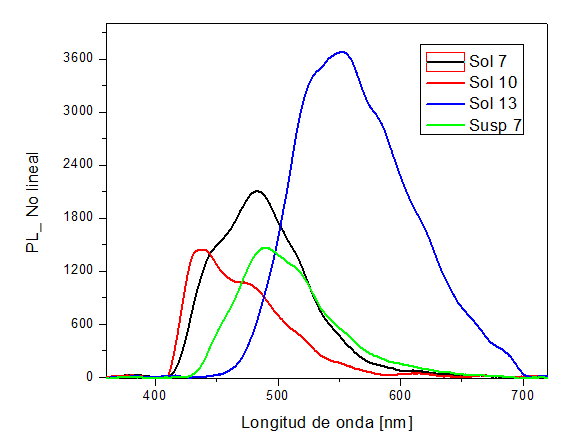
\includegraphics[width=0.85\textwidth]{resultados/sechgo/eminolinhgo}
\caption{Espectros de emisi\'on no lineal de las mol\'eculas 10 y 13 en soluci\'on y 7 en soluci\'on y suspensi\'on (Excitaci\'on a 750 $nm$).}\label{eminlhgo}
\end{figure}

Los valores obtenidos de secci\'on transversal de absorci\'on de dos fotones se muestran graficados en la figura \ref{tpahgo}. La soluci\'on 13 present\'o los valores m\'as altos de $\sigma^{TPA}$ en todas las longitudes de onda de excitaci\'on (menores a 600 $GM$) y el resto de las muestras presentaron valores menores de 300 $GM$. De los materiales org\'anicos con los que se trabajaron en este proyecto, este conjunto de mol\'eculas present\'o algunos de los valores m\'as bajos de eficiencias cu\'anticas de fluorescencia y $\sigma^{TPA}$, adem\'as la mayor\'ia de suspensiones acuosas de nanopart\'iculas se precipitaban inmediatamente despu\'es de ser fabricadas, volviendo las suspensiones m\'as turbias e inestables. Por ello no fue de inter\'es continuar con los estudios de absorci\'on no lineal y utilizar estos materiales como posibles marcadores celulares.



\begin{figure}[H]
\centering
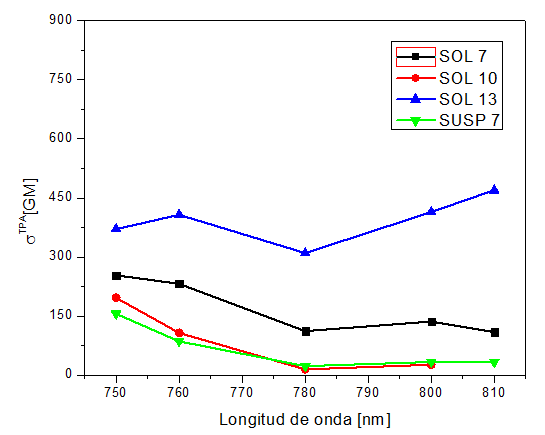
\includegraphics[width=0.85\textwidth]{resultados/sechgo/TPAhgo}
\caption{Epectros de absorci\'on no lineal de las mol\'eculas 10 y 13 en soluci\'on y 7 en soluci\'on y suspensi\'on}\label{tpahgo}
\end{figure}





%. En la figura \ref{X} se muestran los espectros de absorci\'on lineal molar $\epsilon$ de estas soluciones y suspensiones. La mayor absorci\'on se presenta en 
%. En la figura \ref{X} se muestran los espectros de absorci\'on lineal molar $\epsilon$ de estas soluciones y suspensiones. La mayor absorci\'on se presenta en 
%. En la figura \ref{X} se muestran los espectros de absorci\'on lineal molar $\epsilon$ de estas soluciones y suspensiones. La mayor absorci\'on se presenta en 
%. En la figura \ref{X} se muestran los espectros de absorci\'on lineal molar $\epsilon$ de estas soluciones y suspensiones. La mayor absorci\'on se presenta en 
%. En la figura \ref{X} se muestran los espectros de absorci\'on lineal molar $\epsilon$ de estas soluciones y suspensiones. La mayor absorci\'on se presenta en 

\section{Copol\'imero PF2/6-b-P3TMAHT}

Para este copol\'imero, cuya estructura qu\'imica se muestra en la figura \ref{copolimerito}, se realizaron dos soluciones y una suspensi\'on acuosa de nanopart\'iculas bajo condiciones distintas al resto de los materiales del proyecto. Era de inter\'es para este trabajo estudiar las propiedades \'opticas del copol\'imero anfif\'ilico en soluci\'on, utilizando como disolvente una mezcla de agua y THF (el material no es soluble en THF). 

En las dos soluciones realizadas se disolvi\'o el material en un volumen de agua- THF en proporci\'on 1:1 a concentraciones de $9.25 \times 10 ^{-6} M$ y $6.66\times 10^{-8} M$; para elaborar la suspensi\'on, a una concentraci\'on de $6.66\times 10^{-8} M$, se utiliz\'o dodecilsulfato s\'odico (SDS) como surfactante. Se manejaron bajas concentraciones para formar nanoagregados vesiculares y evitar las estructuras de tipo lamelar\cite{scherf}.

En la figura \ref{abscopo} se observan los espectros de absorci\'on molar del copol\'imero en soluciones y en suspensi\'on acuosa. En \'estos se aprecian dos m\'aximos alrededor de 370 y 450 $nm$ correspondientes a los dos bloques o dos distintos mon\'omeros polimerizados que constituyen este copol\'imero.

\begin{figure}[h]
\centering
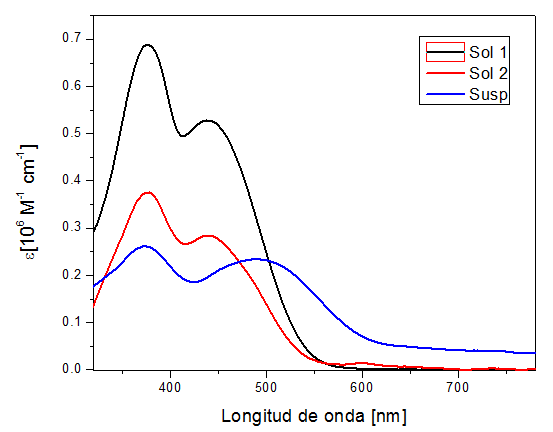
\includegraphics[width=0.85\textwidth]{resultados/copolimero/absmol}
\caption{Espectros de absorci\'on molar de soluciones y suspensi\'on. Concentraciones: \emph{Sol 1}- $9.25 \times 10 ^{-6} M$, \emph{Sol 2}- $6.66\times 10^{-8} M$ y \emph{Susp}- $6.66\times 10^{-8} M$.}\label{abscopo}
\end{figure}

La diferencia entre los espectros de las soluciones 1 y 2 (\emph{Sol 1} y \emph{Sol 2}) radica primordialmente en la intensidad de absorci\'on (Ver Figura \ref{absnormalizadita}), lo cual indica que a ambas concentraciones se forman el mismo tipo de estructuras vesiculares; adem\'as no presentaron esparcimiento. El espectro de la suspensi\'on present\'o una disminuci\'on de la absorci\'on, adem\'as del esparcimiento y un ensanchamiento y corrimiento hacia el rojo del m\'aximo que estaba alrededor de 450 $nm$ (\'unicamente un bloque), esto probablemente se debi\'o a la creciente algomeraci\'on que sufri\'o dicho bloque en el SDS.
 
\begin{figure}[h]
\centering
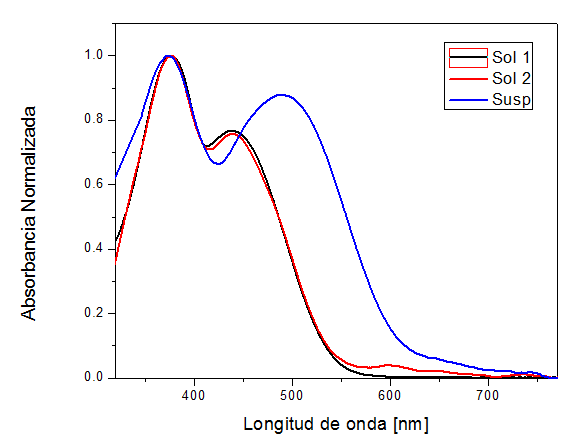
\includegraphics[width=0.65\textwidth]{resultados/copolimero/abs_norm}
\caption{Espectros de absorci\'on molar normalizados para la soluci\'on 1, 2 y una suspensi\'on acuosa.}\label{absnormalizadita}
\end{figure}

Posteriormente se adquirieron los espectros de emisi\'on lineal utilizando un diodo l\'aser como fuente de excitaci\'on, emitiendo a 370 $nm$. La emisi\'on de la suspensi\'on fue muy d\'ebil y no pudo detectarse; en la figura \ref{copoemilineal} se muestran los espectros de emisi\'on de las soluciones a concentraciones de $9.25 \times 10 ^{-6} M$ (\emph{Sol 1}) y $6.66\times 10^{-8} M$ (\emph{Sol 2}). La baja concentraci\'on de la soluci\'on 2 dificult\'o la detecci\'on de emisi\'on, como se muestra en la figura \ref{emilinnorm}, en donde se puede apreciar el ruido o luz de fondo. 

\begin{figure}[H]
\centering
\begin{subfigure}{0.49\textwidth}
\centering
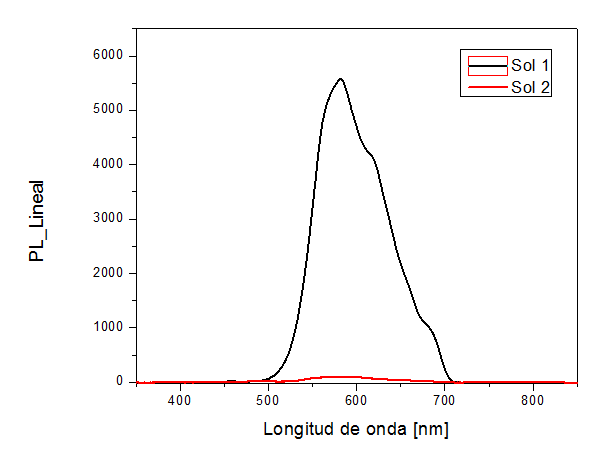
\includegraphics[width=\textwidth]{resultados/copolimero/pl_lineal}\caption{Emisi\'on lineal}\label{}
\end{subfigure}
\begin{subfigure}{0.47\textwidth}
\centering
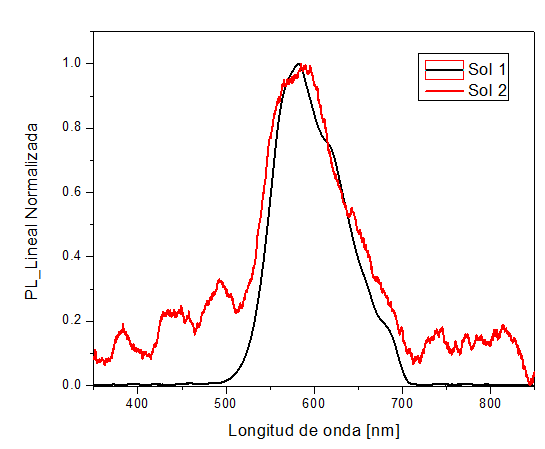
\includegraphics[width=\textwidth]{resultados/copolimero/pl_lineal_norm}\caption{Emisi\'on lineal normalizada}\label{emilinnorm}
\end{subfigure}
\caption{Espectros de emisi\'on lineal del copol\'imero en soluci\'on. Concentraciones: \emph{Sol 1}- $9.25 \times 10 ^{-6} M$ y \emph{Sol 2}- $6.66\times 10^{-8} M$ .}\label{copoemilineal}
\end{figure}

El valor de la eficiencia cu\'antica de fluorescencia ya era conocido, se reporta en la referencia \cite{scherf} y es $\Phi_f=0.16$. Tomando en cuenta lo anterior, finalmente se obtuvieron los espectros de emisi\'on no lineal para determinar la secci\'on transversal de absorci\'on de dos fotones en un rango de excitaci\'on de 760 a 810 $nm$. \'Unicamente se detect\'o la emisi\'on no lineal de la soluci\'on 1 a una concentraci\'on de $9.25 \times 10 ^{-6} M$; en la figura \ref{nolinealejemplos} se muestran algunos espectros de emisi\'on utilizando longitudes de onda de excitaci\'on de 760, 790 y 810 $nm$. Los valores obtenidos de $\sigma ^{TPA}$ de 760 a 810 $nm$ se muestran en la figura \ref{sigmacopo}. 



\begin{figure}[h]
\centering
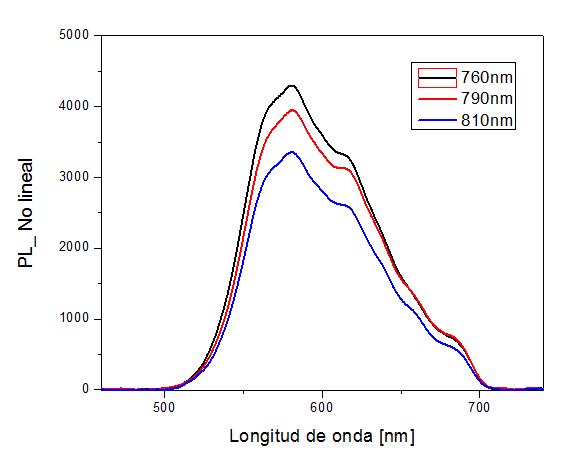
\includegraphics[width=0.69\textwidth]{resultados/copolimero/eminolineal}
\caption{Espectros de emisi\'on no lineal del copol\'imero en soluci\'on. Longitudes de excitaci\'on: 760, 790 y 810 $nm$.}\label{nolinealejemplos}
\end{figure}



\begin{figure}[H]
\centering
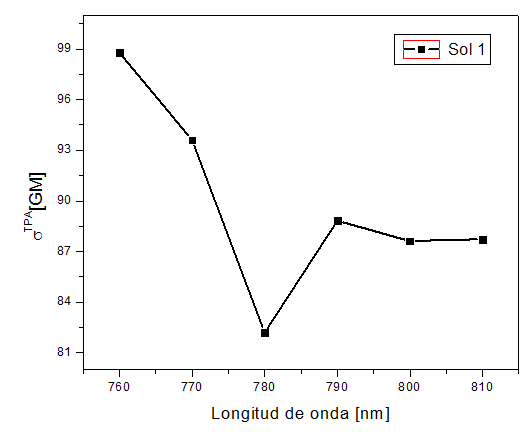
\includegraphics[width=0.68\textwidth]{resultados/copolimero/tpacopo}
\caption{Espectros de absorci\'on no lineal del copol\'imero en soluci\'on, c=$9.25 \times 10 ^{-6} M$.}\label{sigmacopo}
\end{figure}

Como se aprecia en la figura \ref{sigmacopo} hay un valor m\'inimo de $\sigma ^{TPA}$ en 780 $nm$; \'esto probablemente indique la separaci\'on entre los m\'aximos de absorci\'on de los dos bloques. Los valores de secci\'on transversal de absorci\'on de dos fotones para \'este copol\'imero en soluci\'on son muy bajos comparados con la literatura ($10^5 GM$) y con otros materiales estudiados en este trabajo; por ello no se estudi\'o la emisi\'on inducida por absorci\'on de dos fotones en otro rango de excitaci\'on. 
 
 
 


%%%%%%%%%%%%%%%%%%%%%%%%%%%%%%%%%%%%%%%%%%%%%%%%%%%%%%%%%%%%%%%%%%%%%%%%%%%
%%%%%%%%%%%%%%%%%%%%%%%%%%%%%%%%%%%%%%%%%%%%%%%%%%%%%%%%%%%%%%%%%%%%%%%%%%%
%%%%%%%%%%%%%%%%%%%%%%%%%%%%%%%%%%%%%%%%%%%%%%%%%%%%%%%%%%%%%%%%%%%%%%%%%%%
%%%%%%%%%%%%%%%%%%%%%%%%%%%%%%%%%%%%%%%%%%%%%%%%%%%%%%%%%%%%%%%%%%%%%%%%%%%
\section{Comparaci\'on de propiedades \'opticas entre sistemas moleculares dipolar, cuadrupolar y octopolar}

Inicialmente se prepararon soluciones en THF y suspensiones acuosas de nanopart\'iculas para las mol\'eculas 1NDS, 2NQS y 3NOS (Ver Figura \ref{ar2}) a una concentraci\'on de $6.25 \times 10^{-6} M$ utilizando CTAB. En la figura \ref{X} se muestran los espectros de absorci\'on lineal molar $\epsilon$ de estas soluciones y suspensiones. La mayor absorci\'on se presenta en el sistema octopolar, luego en el sistema cuadrupolar y finalmente en el sistema dipolar. 

\begin{figure}[h]
\centering
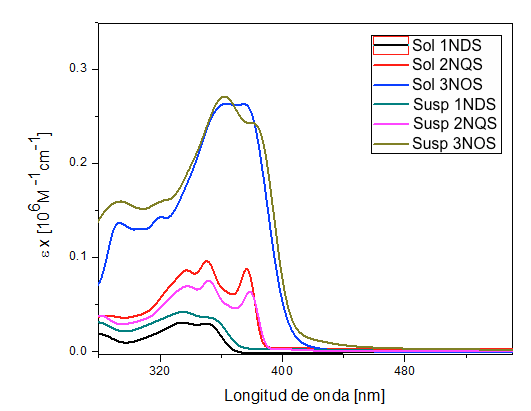
\includegraphics[width=0.85\textwidth]{resultados/sec1/comp}
\caption{Espectros de absorci\'on molar de 1NDS, 2NQS, 3NOS. Las etiquetas \emph{sol} y \emph{susp} se refieren a los sistemas moleculares en soluci\'on y suspensi\'on respectivamente}\label{X}
\end{figure}

Posteriormente se adquirieron los espectros de emisi\'on lineal de las soluciones y suspensiones a la misma concentraci\'on, utilizando un diodo l\'aser de 370 $nm$. Estos espectros se muestran en la figura \ref{los3espemilineal} y se puede apreciar que la mayor emisi\'on se presenta en el sistema octopolar en soluci\'on y en suspensi\'on de nanopart\'iculas. En todos los sistemas moleculares la emisi\'on del material en soluci\'on fue mayor que en suspensi\'on de nanopart\'iculas y en el caso del sistema octopolar 3NOS, el espectro de emisi\'on en suspensi\'on sufri\'o un corrimiento hacia el rojo comparado con el espectro en soluci\'on (Ver Figura \ref{3nsolsusp}); esto se atribuye las interacciones moleculares ocasionadas por el confinamiento del material al formar las nanopart\'iculas.  



\begin{figure}
\centering
\begin{subfigure}{\textwidth}
\centering
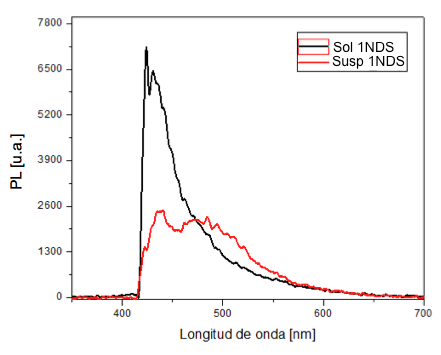
\includegraphics[width=0.65\textwidth]{resultados/sec1/1n}
\end{subfigure}
\begin{subfigure}{\textwidth}
\centering
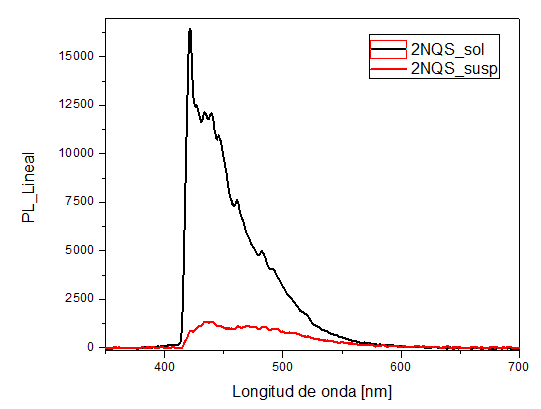
\includegraphics[width=0.65\textwidth]{resultados/sec1/2n}
\end{subfigure}
\begin{subfigure}{\textwidth}
\centering
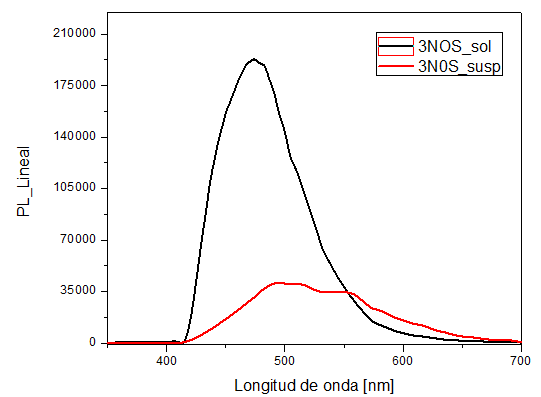
\includegraphics[width=0.65\textwidth]{resultados/sec1/3n}
\end{subfigure}
\caption{Espectros de emisi\'on lineal de 1NDS, 2NQS y 3NOS en soluci\'on y suspensi\'on de nanopart\'iculas}
\label{los3espemilineal}
\end{figure}



\begin{figure}[h]
\centering
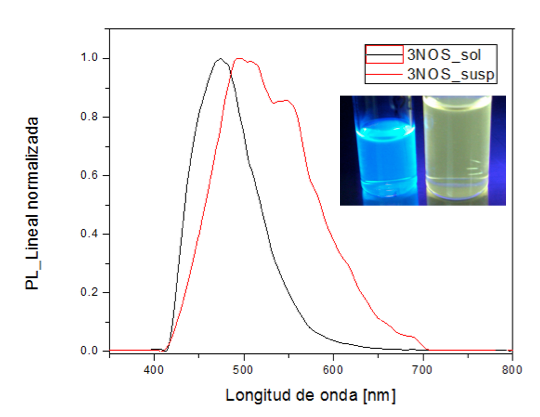
\includegraphics[width=0.85\textwidth]{resultados/sec1/emilinealnorm3N}
\caption{Espectros normalizados y fluorescencia visible de 3NOS en soluci\'on (azul) y suspensi\'on (amarilla)}\label{3nsolsusp}
\end{figure}


En comparaci\'on con el sistema octopolar, la emisi\'on lineal (y no lineal como se ver\'a en seguida) de los sistemas dipolar y cuadrupolar fue muy d\'ebil. Por ello \'unicamente fue de inter\'es medir varias veces la eficiencia cu\'antica de fluorescencia del sistema octopolar 3NOS, en soluci\'on y suspensi\'on acuosa de nanopart\'iculas utilizando CTAB y nuevamente a una concentraci\'on de $6.25 \times 10^{-6} M$; los valores obtenidos utilizando la ecuaci\'on \ref{final} y un factor de correci\'on de 0.6 para la soluci\'on octopolar (por la respuesta del PMT) se muestran en la tabla \ref{tablita}. 

\begin{table}[H]
\centering
\scalebox{0.82}{
\begin{tabular}{| l | c | c | c | c | c | c | c | c | r | }  %p{6.5cm} | c |
\hline
 3NOS           & $\Phi_{f1}$	&$\Phi_{f2}$ &$\Phi_{f3}$&$\Phi_{f4}$&$\Phi_{f5}$& $\Phi_{fPromedio}$&$\Phi_{fPromedio}$ /correcci\'on PMT  \\ \hline   %\multicolumn{8}{|c|}
Soluci\'on &    0.457&	0.539& 0.341	& -	& -	&0.44& 0.26 \\ \hline
Suspensi\'on & 	0.129 &	 0.191& 0.094 & 0.225& 0.226	& 0.17&0.17 \\ \hline
\end{tabular} } 
\caption{ Valores obtenidos de eficiencia cu\'antica de fluorescencia $\Phi$ para el sistema octopolar  \label{tablita}}
\end{table}


Las mediciones de $\sigma^{TPA}$ en el rango de 740 $nm$ a 840 $nm$ para los tres sistemas moleculares se realizaron a una concentraci\'on de $6.25\times 10^{-6} M$. A esta concentraci\'on los espectros de emisi\'on no lineal de los sistemas dipolar y cuadrupolar tanto en soluci\'on como en suspensi\'on estuvieron por debajo del nivel de detecci\'on del arreglo experimental (Ver Figura \ref{nel}); sin embargo, los espectros del sistema octopolar para algunas longitudes de onda de excitaci\'on se muestran en la figura \ref{sip} y los valores de $\sigma^{TPA}$ se presentan en la gr\'afica de la figura \ref{tpaprimeros}.

\begin{figure}
\centering
\begin{subfigure}{\textwidth}
\centering
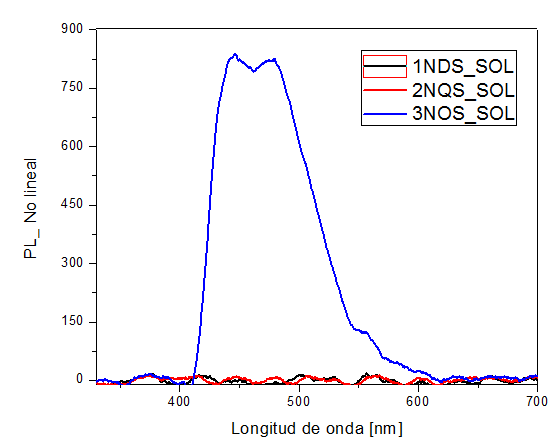
\includegraphics[width=0.6\textwidth]{resultados/sec1/nojalo}
\caption{Espectros de emisi\'on no lineal para 1NDS, 2NQS y 3NOS en soluci\'on con un haz de excitaci\'on a 760 $nm$ }\label{nel}
\end{subfigure}
\begin{subfigure}{\textwidth}
\centering
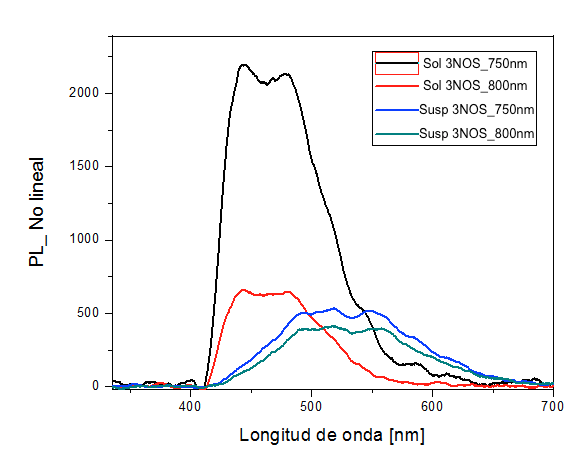
\includegraphics[width=0.7\textwidth]{resultados/sec1/sijalo}
\caption{Comparaci\'on de espectros de emisi\'on no lineal para 3NOS en soluci\'on y suspensi\'on para diferentes longitudes de onda de excitaci\'on }\label{sip}
\end{subfigure}
\caption{Espectros de emisi\'on no lineal}
\label{ghghh}
\end{figure}

\begin{figure}[h]
\centering
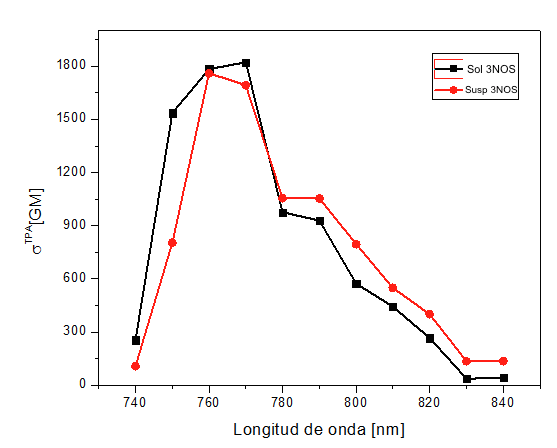
\includegraphics[width=0.7\textwidth]{resultados/sec1/TPA_1}
\caption{Espectro de absorci\'on no lineal de 3NOS en soluci\'on y suspensi\'on}\label{tpaprimeros}
\end{figure}

Posteriormente se realizaron pruebas para recubrir las nanopart\'iculas de la mol\'ecula octopolar con PEG 5000 sin utilizar surfactantes. Se prepar\'o una suspensi\'on acuosa de nanopart\'iculas a una concentraci\'on de $6.43 \times 10^{-6}M$, utilizando una concentraci\'on de PEG 5000 de $5\times 10^{-6} M$. En la figura \ref{grr} se muestra una comparaci\'on de los espectros de absorci\'on (\ref{abspeg1}) y emisi\'on lineal (\ref{emipeg1}) de la mol\'ecula octopolar en soluci\'on, suspensi\'on utilizando CTAB y suspensi\'on de nanopart\'iculas utilizando PEG 5000, todas a la misma concentraci\'on $6.43 \times 10^{-6}M$. 

\begin{figure}
\centering
\begin{subfigure}{0.5\textwidth}
\centering
\includegraphics[width=\textwidth]{resultados/sec1/abs_peg5000}
\caption{Absorci\'on molar lineal }\label{abspeg1}
\end{subfigure}
\begin{subfigure}{0.49\textwidth}
\centering
\includegraphics[width=\textwidth]{resultados/sec1/emi_peg5000}
\caption{Emisi\'on lineal }\label{emipeg1}
\end{subfigure}
\caption{Espectros de la mol\'ecula octopolar en soluci\'on \emph{Sol} y  en suspensiones con CTAB \emph{Susp CTAB} y PEG \emph{Susp PEG 5000}}
\label{grr}
\end{figure}

Se realizaron cinco mediciones de eficiencia cu\'antica de fluorescencia para la suspensi\'on acuosa de nanopart\'iculas funcionalizadas con PEG 5000 obteniendo una eficiencia promedio $\Phi_{f_{Promedio}}$ de 0.14. Tambi\'en se midi\'o la secci\'on transversal de absorci\'on de dos fotones de esta suspensi\'on para las siguientes longitudes de onda de excitaci\'on: 760, 780, 800 y 815 $nm$; los valores de $\sigma^{TPA}$ se muestran en la figura \ref{valoressigmapeg1}.

\begin{figure}[H]
\centering
\includegraphics[width=0.7\textwidth]{resultados/sec1/TPA_PEG1}
\caption{Espectro de absorci\'on no lineal para 3NOS en soluci\'on \emph{Sol} y suspensiones con CTAB \emph{Susp CTAB} y PEG 5000, \emph{Susp PEG 5000}}\label{valoressigmapeg1}
\end{figure}

En este trabajo la mol\'ecula octopolar fue uno de los sistemas moleculares  de mayor inter\'es, por ello se determinaron los valores de $\sigma^{TPA}$ en el rango de longitudes de onda incidentes de 650 a 760 $nm$ implementando el arreglo \'optico de TPEF como se explic\'o en la secci\'on \ref{laserchidote}. En este rango se determin\'o $\sigma^{TPA}$ para la mol\'ecula 3NOS en soluci\'on a una concentraci\'on de $6.43 \times 10^{-6} M$; sin embargo, debido a la sensibilidad del arreglo y al nivel de detecci\'on, a ciertas longitudes de onda no pudo determinarse $\sigma^{TPA}$. Los resultados se muestran en la figura \ref{valoressigmafs} junto con los resultados obtenidos anteriormente para la soluci\'on en el primer rango, de 740 a 840 $nm$ (Ver Figura \ref{tpaprimeros}).

Posteriormente se realiz\'o una funcionalizaci\'on de nanopart\'iculas de la mol\'ecula octopolar, utilizando ahora el PEG 2000. Se prepar\'o una suspensi\'on acuosa de nanopart\'iculas sin CTAB a una concentraci\'on de $6.43 \times 10^{-6} M$ y con una concentraci\'on de PEG 2000 en la suspensi\'on de $6\times 10^{-4} M$. En la figura \ref{temi} se muestran un par de im\'agenes de esta suspensi\'on adquiridas con un microscopio electr\'onico de transmisi\'on o TEM por sus siglas en ingles, de la marca Philips modelo XL; los di\'ametros de las nanopart\'iculas van de 16.8 a 33.7 $nm$. 


\begin{figure}[H]
\centering
\includegraphics[width=0.7\textwidth]{resultados/sec1/TPA_femto}
\caption{Espectros de absorci\'on no lineal para 3NOS en soluci\'on de 650--760 nm y de $740-840nm$}\label{valoressigmafs}
\end{figure}

\begin{figure}[H]
\centering
\includegraphics[width=\textwidth]{resultados/sec1/tem}
\caption{Im\'agenes TEM con escala de 20 y 500 $nm$}\label{temi}
\end{figure}

El PEG 2000 facilita la funcionalizaci\'on de nanopart\'iculas porque tiene m\'as grupos funcionales que el PEG 5000 como se mencion\'o en la secci\'on \ref{pegis}, adem\'as las suspensiones fabricadas con PEG 2000 fueron m\'as estables; en un tiempo de almacenamiento de m\'as de cinco meses a temperatura ambiente la suspensi\'on de nanopart\'iculas de 3NOS no se precipit\'o. Por ello y por las propiedades \'opticas que present\'o la mol\'ecula octopolar se decidi\'o internalizar esta suspensi\'on acuosa de nanopart\'iculas funcionalizadas con PEG 2000 en la l\'inea celular X.

Se internalizaron 500 $\mu l$ de la suspensi\'on a una concentraci\'on de $6.43 \times 10^{-6} M$ ...  


\section{Nanopart\'iculas del pol\'imero PMC300} 

La caracterizaci\'on \'optica de este pol\'imero, cuya estructura se muestra en la figura \ref{PMC}, fue una de las m\'as amplias de este trabajo. Se fabricaron soluciones de PMC300 y de PMC300 dopado con Rodamina 6G en THF; se fabricaron tambi\'en suspensiones acuosas de nanopart\'iculas de PMC300 y de PMC300 dopado con Rodamina 6G, utilizando para algunos casos CTAB y para otros una funcionalizaci\'on con PEG 2000 (recubrimiento). Este pol\'imero ya ha sido estudiado en soluci\'on y en suspensi\'on (utilizando CTAB como surfactante) por el GMPOM\footnote{En particular el PMC300 fue estudiado por la Dra. Laura Aparicio Ixta, ver referencia \cite{laurita}}; por ello en este trabajo, el estudio del pol\'imero se enfoc\'o en las nanopart\'iculas funcionalizadas con PEG 2000.

En la figura \ref{pmc_abs1} se muestran los espectros de absorci\'on molar de las soluciones y suspensiones estudiadas para este pol\'imero. La etiqueta \emph{Sol PMC300} hace referencia a la soluci\'on del pol\'imero, \emph{Susp PMC300} indica que se trata de la suspensi\'on acuosa del pol\'imero precursor funcionalizada con PEG 2000, \emph{Sol PMC300/Rod 6G} se refiere a la soluci\'on de PMC300 dopada con Rodamina 6G al 177\% molar y \emph{Susp PMC300/Rod 6G} es el espectro de la suspensi\'on acuosa de nanopart\'iculas con PEG 2000; se manejaron concentraciones bajas de PMC300, del orden de $10^{-7} M$.


\begin{figure}[H]
\centering
\includegraphics[width=0.85\textwidth]{resultados/pmc300/abs1}
\caption{Espectros de absorci\'on molar de soluciones y suspensiones acuosas de PMC300 y PMC300/Rodamina 6G}\label{pmc_abs1}
\end{figure}

En \'estos espectros de absorci\'on molar se pueden apreciar dos m\'aximos alrededor de 330 y y 435 $nm$ correspondientes al pol\'imero PMC300; en el caso de las muestras que se prepararon solo con PMC300, la suspensi\'on present\'o tanto esparcimiento como un ligero corrimiento hacia el rojo de uno de los m\'aximos en comparaci\'on con la soluci\'on. Para la soluci\'on y suspensi\'on de PMC300 dopada con Rodamina 6G al 177\% molar, se present\'o una disminuci\'on en la intensidad de absorci\'on y nuevamente un corrimiento hacia el rojo de uno de los m\'aximos en la suspensi\'on; alrededor de 520 $nm$ se aprecia la absorci\'on correspondiente a la Rodamina 6G.

Las muestras de PMC300 dopadas con Rodamina 6G a diferentes concentraciones, tanto en soluci\'on como en suspensi\'on, se realizaron para estudiar y optimizar la transferencia de energ\'ia tipo F\"orster. En la figura \ref{}










\chapter{Conclusiones}   %\label{chap_content}



Para medir eficiencia cu\'antica de fluorescencia, en ocasiones no se contaba con el amplificador lock- in y se realizaron pruebas utilizando un mult\'imetro.




investigar el tiempo de vida de los materiales organicos


On the contrary, at low temperatures and/or in a rigid medium, phosphorescence
can be observed.


% A pesar de que se trabaj\'o con la soluci\'on de concentraci\'on mayor (Soluci\'on 1, c= $9.25 \times 10 ^{-6} M$), se mostr\'o con los espectros de absorci\'on y emisi\'on lineales, que se obtienen las mismas estructuras vesiculares que a menores concentraciones. 
%CONCLUSIONES -------^

\appendix
\chapter[C\'alculo del factor de correccion para \texorpdfstring{$\Phi_f$}{Phif}]{Factor de correcci\'on para la eficiencia cu\'antica de fluorescencia}{}\label{apendicitis} %\vspace{-30pt}

%\includegraphics[height=0.90\textheight]{appendices/app-thesis}
%\chapter{Ap\'endices}
%\section{C\'alculo del factor de correccion del PMT}\label{apendicitis} 

En la figura \ref{kk} se muestra la curva de sensibilidad de respuesta contra longitud de onda que tiene el PMT modelo R7400U-01. 

Cuando la fluorescencia de la muestra de inter\'es y de la referencia (Rodamina 6G) tienen longitudes de onda similares, el PMT responder\'a de la misma manera en ambas muestras; sin embargo, si la muestra y la referencia emiten en diferentes longitudes de onda es necesario considerar un factor de correcci\'on.

Inicialmente se consider\'o que para la Rodamina 6G, la longitud de onda en la que se presenta la m\'axima emisi\'on es de 600 $nm$. El factor de correcci\'on se determin\'o calculando la raz\'on entre el valor de sensibilidad a 600 $nm$ y el valor de sensibilidad a la longitud de onda de mayor emisi\'on de la muestra de inter\'es. Finalmente para obtener el valor m\'as preciso de $\Phi_f$ se multiplic\'o el factor de correcci\'on por el valor de $\Phi_f$ que se obtiene sin tomar en cuenta la curva de sensibilidad del PMT. 

Por ejemplo, para el caso de la mol\'ecula octopolar en soluci\'on de THF, la cual emit\'ia en azul (450 $nm$), el factor de correcci\'on fue 0.6 o bien $30/50$ que son los valores de sensibilidad a 600 y 450 $nm$ respectivamente. Este valor se multiplic\'o por $\Phi_{fPromedio}=0.44$ para obtener $\Phi_f=0.26$ como se indic\'o en la tabla \ref{tablita}.

\begin{figure}[h]
\centering
\includegraphics[width=0.85\textwidth]{appendices/pmtsensi}
\caption{Sensibilidad de respuesta del PMT. \emph{\scriptsize{Imagen adquirida de la hoja de especificaciones del PMT marca HAMAMATSU modelo R7400U-01.}}}\label{kk}
\end{figure}




 %es necesario introducir un factor de correci\'on.


%\footnote{Este factor de correcci\'on se obtiene de las curvas de respuesta del PMT contenidas el manual de dicho equipo} 




\backmatter
%\chapter{Ap\'endices}

\section{C\'alculo del factor de correccion del PMT}\label{apendicitis} 
 Cuando la fluorescencia de la muestra de inter\'es y de la referencia (Rodamina 6G) tienen longitudes de onda similares, el PMT responder\'a de la misma manera en ambas muestras; sin embargo, si la muestra y la referencia emiten a diferentes longitudes de onda no tendr\'an la misma respuesta 







 es necesario introducir un factor de correci\'on.


\footnote{Este factor de correcci\'on se obtiene de las curvas de respuesta del PMT contenidas el manual de dicho equipo} 







\clearpage
\thispagestyle{empty}

%%%%%%%%%%%%%%%%%%%%%%%%% Select one bibliography style %%%%%%%%%%%%%%%%%%%%%%%%%%%%
%\bibliographystyle{plain}
%\bibliographystyle{abbrv}
%\bibliographystyle{alpha}
\bibliographystyle{unsrt}
\nocite{*} 
\bibliography{base/thesis}




\end{document}
